\documentclass[11pt]{article}

% Change "review" to "final" to generate the final (sometimes called camera-ready) version.
% Change to "preprint" to generate a non-anonymous version with page numbers.
\usepackage[preprint]{acl}
% Standard package includes
\usepackage{times}
\usepackage{latexsym}
% For proper rendering and hyphenation of words containing Latin characters (including in bib files)
\usepackage[T1]{fontenc}
% For Vietnamese characters
% \usepackage[T5]{fontenc}
% See https://www.latex-project.org/help/documentation/encguide.pdf for other character sets

% This assumes your files are encoded as UTF8
\usepackage[utf8]{inputenc}

% This is not strictly necessary, and may be commented out,
% but it will improve the layout of the manuscript,
% and will typically save some space.
\usepackage{microtype}

% This is also not strictly necessary, and may be commented out.
% However, it will improve the aesthetics of text in
% the typewriter font.
\usepackage{inconsolata}
\usepackage{fontspec}
\newfontfamily\hindifont{Noto Sans Devanagari}
% Including images in your LaTeX document requires adding
% additional package(s)
\usepackage{graphicx}

% Additional packages for the skeleton
\usepackage{booktabs}       % professional tables (\toprule, \midrule, \bottomrule)
\usepackage{multirow}       % multi-row table cells
\usepackage{tabularx}       % flexible-width tables
\usepackage{amsmath}        % math environments
\usepackage{amssymb}        % math symbols
\usepackage{xcolor}         % colored text for TODO notes
\usepackage{enumitem}       % customise list spacing

% If the title and author information does not fit in the area allocated, uncomment the following
%
%\setlength\titlebox{<dim>}
%
% and set <dim> to something 5cm or larger.

% ---------------------------------------------------------------
% Useful commands for filling in the skeleton
% ---------------------------------------------------------------
\newcommand{\eg}{\textit{e.g.,}\ }
\newcommand{\ie}{\textit{i.e.,}\ }
\newcommand{\etal}{\textit{et al.}}
% Use \TODO{} to mark sections that still need content (shows in red)
\newcommand{\TODO}[1]{\textcolor{red}{\textbf{[TODO: #1]}}}
% Use \NOTE{} to leave yourself internal notes (shows in blue)
\newcommand{\NOTE}[1]{\textcolor{blue}{\textit{[NOTE: #1]}}}

% ---------------------------------------------------------------
% TITLE
% ---------------------------------------------------------------
\title{Mathematical Reasoning Under Token Budgets: Mathematical Accuracy and Script Usage Across Indic Languages}

% ---------------------------------------------------------------
% AUTHORS
% ---------------------------------------------------------------
% For several authors from the same institution:
\author{Ashish Shetty \and Gagan Singh \and Manmay Maheshwari  \and S Rishab \\
        BITS Pilani, Pilani Campus}
% if the names do not fit well on one line use
%         Author 1 \\ {\bf Author 2} \\ ... \\ {\bf Author n} \\
% For authors from different institutions:
% \author{Author 1 \\ Address line \\  ... \\ Address line
%         \And  ... \And
%         Author n \\ Address line \\ ... \\ Address line}
% To start a separate ``row'' of authors use \AND, as in
% \author{Author 1 \\ Address line \\  ... \\ Address line
%         \AND
%         Author 2 \\ Address line \\ ... \\ Address line \And
%         Author 3 \\ Address line \\ ... \\ Address line}

% \author{Anonymous Submission}

%\author{
%  \textbf{First Author\textsuperscript{1}},
%  \textbf{Second Author\textsuperscript{1,2}},
%  \textbf{Third T. Author\textsuperscript{1}},
%  \textbf{Fourth Author\textsuperscript{1}},
%\\
%  \textbf{Fifth Author\textsuperscript{1,2}},
%  \textbf{Sixth Author\textsuperscript{1}},
%  ...
%\\
%  \textsuperscript{1}Affiliation 1,
%  \textsuperscript{2}Affiliation 2
%\\
%  \small{
%    \textbf{Correspondence:} \href{mailto:email@domain}{email@domain}
%  }
%}

% ===============================================================
\begin{document}
\maketitle
% ===============================================================

% ---------------------------------------------------------------
% ABSTRACT
% ---------------------------------------------------------------
% Instructions: 150-250 words. No citations. Cover four points:
%   (1) Problem statement  (2) Research gap
%   (3) Approach           (4) Key experimental result
% ---------------------------------------------------------------
\begin{abstract}
We study whether fixed reasoning-token budgets affect mathematical reasoning differently across English and ten Indic languages. We evaluate DeepSeek-R1-Distill-Qwen-1.5B on Sarvam AI's GSM8K-Indic dataset, using the same 200 underlying questions across eleven language conditions and five reasoning-token budgets: 50, 100, 200, 400, and 800. This yields 11,000 generations. We measure exact-match accuracy, natural finish rate, character-level target-script ratio, and token bloat relative to English among naturally completed thinking traces at the 800-token budget. English accuracy increases from 21\% at 50 tokens to 64\% at 800 tokens. Hindi has the highest accuracy among the Indic languages, increasing from 5.5\% to 24\%. Gujarati has the highest average token-bloat multiplier relative to English (2.85$\times$), the strongest target-script persistence, and a notably low natural finish rate. Marathi has the lowest measured token-bloat multiplier (1.54$\times$). These results show language-dependent differences in accuracy, completion, and token usage under a shared budget. They do not establish that token bloat causes lower accuracy. The current evaluation covers one model; evaluating additional models remains future work.
\end{abstract}
% ---------------------------------------------------------------
% 1. INTRODUCTION
% ---------------------------------------------------------------
\section{Introduction}
\label{sec:intro}

Large language models (LLMs) are increasingly used for tasks that require mathematical and logical reasoning. These models can generate intermediate reasoning steps before producing a final answer \citep{wei2022chain, openai2024o1}. However, their performance can vary across languages. Previous evaluations have reported differences between English and non-English reasoning performance \citep{shi2022language, goyal2026mindthecap}. These differences raise questions about whether LLMs provide comparable reasoning capabilities across linguistic populations.

Recent methods aim to reduce the computational cost of reasoning by controlling the length of generated responses \citep{aggarwal2025l1, hou2025thinkprune}. These methods often impose length constraints or penalties on generated reasoning. Under a fixed budget, cross-language differences in tokenization can affect how much reasoning text fits within the same limit. Studies have reported inefficiencies in tokenization for non-Latin scripts, including Indic scripts \citep{srivastava2026tokenizertax, shravan2026brahmic}. Consequently, a mathematical problem may require a longer generated sequence in one language than in another. When the available budget is insufficient, a model may stop generating before completing its reasoning or producing a final answer. This raises the question of how tokenization and generation limits affect mathematical reasoning across languages.

Prior research has examined methods for reducing reasoning length and controlling the number of generated tokens \citep{liu2026laser, shorterbetter2025}. Other work benchmarks low-resource Indic languages and studies cross-lingual compression of mathematical reasoning traces \citep{maheshwari2025indicparam, wan2026mcd, dipta2026ganitllm}. A recent study also shows that output-budget choices can change measured multilingual reasoning gaps \citep{goyal2026mindthecap}. However, the relationship between token budgets, target-script usage, generation completion, and mathematical accuracy across Indic languages requires further investigation. In particular, it remains necessary to examine whether script usage is associated with reasoning performance under different generation limits.

We investigate these questions by evaluating mathematical reasoning across ten Indic languages and English. We use the Sarvam GSM8K-Indic dataset, which provides translated versions of GSM8K for ten Indic languages, and evaluate the DeepSeek-R1-Distill-Qwen-1.5B model \citep{sarvam_gsm8k_indic, cobbe2021gsm8k, deepseek2025r1}. We consider five token budgets of 50, 100, 200, 400, and 800 tokens. At each budget, we measure exact-match answer accuracy and whether the generated reasoning finishes naturally or reaches the imposed limit. We also analyze target-script usage through a character-level metric that estimates the proportion of generated reasoning characters belonging to the target script. This analysis allows us to examine how script usage and generation completion vary across languages and token budgets.

We address three research questions: (RQ1) How does exact-match mathematical accuracy change across reasoning-token budgets in English and Indic languages? (RQ2) Is the relative token cost of Indic-language thinking traces associated with natural completion and accuracy? (RQ3) How is target-script usage associated with mathematical accuracy across languages?

Our experiments show that mathematical accuracy and natural completion rates generally improve as the token budget increases, although the size of the improvement varies across languages. For example, from the smallest to the largest budget, English accuracy increases from 21\% to 64\%, while Hindi accuracy increases from 5.5\% to 24\%. The relationship between target-script usage and accuracy is not uniform across languages. Gujarati has the strongest target-script persistence among the Indic languages, but Hindi achieves the highest Indic-language accuracy. These findings indicate that script usage alone does not consistently predict mathematical reasoning accuracy. They motivate further investigation into language-sensitive evaluation methods that account for token usage and generation limits.

\paragraph{Contributions.}
Our contributions are threefold:
\begin{itemize}
    \item \textbf{Budget-based multilingual evaluation:} We evaluate DeepSeek-R1-Distill-Qwen-1.5B on the same 200 underlying GSM8K questions across English and ten Indic languages, using five reasoning-token budgets.
    \item \textbf{Completion and script analysis:} We measure natural finish rates and character-level target-script ratios to characterize how generation completion and script composition vary across languages and budgets.
    \item \textbf{Token-bloat analysis:} We compare token counts for paired English and Indic-language thinking traces that finish naturally at the 800-token budget, and analyze their relationship with language-specific accuracy and completion.
\end{itemize}
% ---------------------------------------------------------------
% 2. RELATED WORK
% ---------------------------------------------------------------
% Instructions:
%   - 2-3 thematic sub-sections covering different categories of prior work.
%   - Each sub-section: discuss 5-10 papers grouped by theme or approach.
%   - END every sub-section with an explicit statement of how your work
%     differs or what gap it fills. This is mandatory.
% ---------------------------------------------------------------
% ---------------------------------------------------------------
% 2. RELATED WORK
% ---------------------------------------------------------------
\section{Related Work}
\label{sec:related}

\subsection{Efficient Reasoning and Length Constraints}
\label{sec:related_cat1}

Recent works train language models to reduce the length of reasoning traces. Researchers apply hard token caps during training or penalize long responses using reinforcement learning \citep{aggarwal2025l1, hou2025thinkprune}. Adaptive methods shape rewards based on sequence length and problem difficulty \citep{liu2026laser, shorterbetter2025}. Other methods enforce strict budget constraints during inference \citep{muennighoff2025s1}. These methods study the trade-off between reasoning length, computational cost, and task performance. Our evaluation asks a related but different question: how does a shared hard reasoning-token budget behave across languages whose generated traces may differ in token cost? 

\noindent\textbf{Gap addressed by this paper:}
A fixed token cap allocates the same number of tokens to each language, regardless of how many tokens a generated trace requires. We measure how completion and accuracy vary under this shared cap rather than assuming that a fixed token count represents an equal amount of reasoning across languages.

\subsection{Multilingual Reasoning Capabilities}
\label{sec:related_cat2}

Language models exhibit significant performance drops when reasoning in non-English languages \citep{shi2022language, goyal2026mindthecap}. The MGSM benchmark measures chain-of-thought reasoning across ten languages using translated grade-school math questions \citep{shi2022language}. More recent work studies how output-budget choices affect measured multilingual reasoning gaps \citep{goyal2026mindthecap}. Other work explores cross-lingual chain-of-thought compression and language-specific mathematical reasoning, including Bengali reasoning models \citep{wan2026mcd, dipta2026ganitllm}. Our study complements this work by measuring answer accuracy, completion, and target-script usage under the same set of hard reasoning-token budgets.

\noindent\textbf{Gap addressed by this paper:}
Our analysis does not assume that either English fallback or native-script reasoning is universally preferable. Instead, we compare target-script usage with accuracy and completion across language conditions.

\subsection{Tokenizer Inefficiency and Sequence Bloat}
\label{sec:related_cat3}

Standard tokenizers struggle to encode non-Latin scripts efficiently. Studies document a severe tokenization penalty for Indic languages \citep{srivastava2026tokenizertax, shravan2026brahmic}. Recent work quantifies differences in tokenization cost for Indian languages and proposes tokenizer designs that improve coverage of Indic scripts \citep{srivastava2026tokenizertax, shravan2026brahmic}. Separate multilingual output-budget analyses show that language-level performance gaps can change with the imposed generation limit \citep{goyal2026mindthecap}. These findings motivate measuring token usage and task performance together under controlled budgets.

\noindent\textbf{Gap addressed by this paper:}
Existing work quantifies tokenizer costs or evaluates multilingual reasoning under output budgets. We complement these studies by measuring target-script composition, natural completion, and accuracy for question-matched English and Indic-language traces under five reasoning-token budgets. These measurements show associations but do not isolate causal effects.

% ---------------------------------------------------------------
% 3. METHODOLOGY
% ---------------------------------------------------------------
% Instructions:
%   - Describe WHAT you did at a conceptual level.
%   - Do NOT include code-level details (no library names, function names,
%     Python code, etc.).
%   - Include a system/block diagram (Figure 1) --- MANDATORY.
%     Use tools like Napkin AI, Excalidraw, or draw.io for a first draft.
%   - The diagram should be colorful and visually appealing.
% ---------------------------------------------------------------

% ---------------------------------------------------------------
% 3. METHODOLOGY
% ---------------------------------------------------------------
% ---------------------------------------------------------------
% 3. METHODOLOGY
% ---------------------------------------------------------------
\section{Methodology}
\label{sec:method}

\subsection{Overview}
\label{sec:method_overview}

We evaluate mathematical reasoning under constrained generation budgets across ten Indic languages and English. Our experiments use the DeepSeek-R1-Distill-Qwen-1.5B model and GSM8K-derived mathematical reasoning datasets. For each question, the model generates an intermediate reasoning trace under a specified token budget. We then prompt the model to produce a final answer using a language-specific answer trigger. We assess mathematical accuracy and analyze reasoning completion and native-script usage across languages and budgets.

\subsection{Dataset Selection}
\label{sec:method_dataset}

We use Sarvam AI's GSM8K-Indic dataset, which provides translated versions of the GSM8K mathematical reasoning benchmark \citep{sarvam_gsm8k_indic, cobbe2021gsm8k}. GSM8K contains grade-school mathematical word problems that require multistep reasoning. We evaluate Bengali, Gujarati, Hindi, Kannada, Malayalam, Marathi, Odia, Punjabi, Tamil, and Telugu, with English as the reference condition. We also evaluate the original English benchmark as a reference for cross-lingual comparisons.

Using translated versions of the same benchmark allows us to study how language variation affects reasoning performance on mathematically related problems. We retain the reference answer associated with each question to evaluate the model's final numerical prediction. This setup supports comparisons across languages while recognizing that translation differences may introduce variation in the linguistic presentation of a problem.

\subsection{Budget-Constrained Reasoning Generation}
\label{sec:method_generation}

We evaluate the DeepSeek-R1-Distill-Qwen-1.5B model under five maximum generation budgets of 50, 100, 200, 400, and 800 tokens. Each question is evaluated separately at every budget. We use deterministic generation settings throughout the experiments.

The model first generates a reasoning trace under the selected budget. If the trace contains the reasoning termination marker \texttt{</think>}, we retain the text preceding that marker and classify the trace as naturally completed. If the marker does not appear before the token limit is reached, we retain the generated trace and classify it as budget-truncated.

This procedure allows us to distinguish traces that reach the model's reasoning termination marker from traces that exhaust their available generation budget. We record this completion status for each question, language, and budget combination.

\subsection{Final Answer Generation and Evaluation}
\label{sec:method_answer}

During initial generation, the model receives only the mathematical question in the target language's native script, with no separate instruction prompt. After the reasoning stage stops, we append a language-specific final-answer trigger in that script. For example, the English trigger is ``Final Answer:'', while the Hindi trigger is ``{\hindifont अंतिम उत्तर:}''.

We allow up to 15 additional tokens for the final-answer stage. These tokens are separate from the reasoning-token budget. We extract the predicted numerical answer from the generated \texttt{\textbackslash boxed\{\}} expression after the trigger. The parser removes dollar signs and commas, extracts numeric substrings, selects the first number, and converts the parsed prediction to an integer. We compare that value with the dataset's already-normalized numeric reference answer. Accuracy is calculated separately for each language and reasoning budget.

\subsection{Character-Level Native Script Tracking}
\label{sec:method_script}

We analyze the character composition of each generated reasoning trace to measure the extent to which the model uses the target script. Let $C_{\text{native}}$ denote the number of counted characters assigned to the target script. Let $C_{\text{counted}}$ denote the total number of counted characters after excluding digits, whitespace, and punctuation from the retained reasoning trace.

We define the native script ratio $R$ as

\begin{equation}
    R = \frac{|C_{\text{native}}|}{|C_{\text{counted}}|} \times 100,
    \label{eq:ratio}
\end{equation}

where $R$ represents the percentage of counted characters in the trace that belong to the target script. A higher value indicates greater use of that script among counted characters. The metric measures script composition and does not identify the semantic language of every word.

We calculate this ratio for each reasoning trace and compare it across languages and token budgets. This analysis helps us examine the relationship between target-script usage, reasoning completion, and mathematical accuracy. The metric measures script composition and does not independently establish the language or meaning of every generated word.

\subsection{Experimental Design}
\label{sec:method_design}
Our experimental design varies the maximum reasoning-trace budget while keeping the model and generation procedure fixed. We evaluate five budgets for each question and record the final-answer accuracy, reasoning completion status, and native script ratio.

We analyze three outcomes. First, we measure how mathematical accuracy changes as the reasoning budget increases. Second, we examine the frequency of naturally completed and budget-truncated traces. Third, we investigate the relationship between native script ratios and final-answer accuracy across languages. Together, these analyses characterize how constrained reasoning generation relates to mathematical performance and script usage in Indic languages.
% ---------------------------------------------------------------
% 4. EXPERIMENTAL SETUP
% ---------------------------------------------------------------
% Instructions:
%   - Use tables for datasets, models, metrics, and baselines.
%   - Every dataset, model, metric, and baseline MUST be cited.
%   - Follow the table formatting of the ACL template (hline or booktabs).
% ---------------------------------------------------------------

\section{Experimental Setup}
\label{sec:experimental_setup}

\subsection{Dataset and Language Coverage}
\label{sec:dataset_language}

We use Sarvam AI's GSM8K-Indic dataset for our multilingual mathematical reasoning experiments \citep{sarvam_gsm8k_indic}. The dataset provides GSM8K mathematical problems in English and ten Indic languages: Bengali, Gujarati, Hindi, Kannada, Malayalam, Marathi, Odia, Punjabi, Tamil, and Telugu. These language versions allow us to investigate how language affects mathematical reasoning under constrained token budgets.

Our evaluation covers eleven language conditions, including English as the reference condition. For each language, we select the same set of 200 questions and evaluate the model at five reasoning-token budgets: 50, 100, 200, 400, and 800 tokens. The same questions are reused across all five budgets within each language, enabling comparisons under different token constraints while keeping the question set fixed.

Each language therefore contributes 1,000 generations, resulting in 11,000 generations across all eleven language conditions. This experimental design supports comparisons of mathematical accuracy and generation completion across languages and token budgets.

As summarized in Figure~\ref{fig:experimental_pipeline}, the evaluation pipeline applies the selected token budget during reasoning generation and then evaluates the extracted final answer. We use exact-match accuracy, character-level target-script ratio, and token bloat relative to English to study answer correctness, script usage, and tokenization differences, respectively. The following subsections describe the model, generation procedure, and evaluation metrics in detail.

\begin{figure}[htbp]
    \centering
    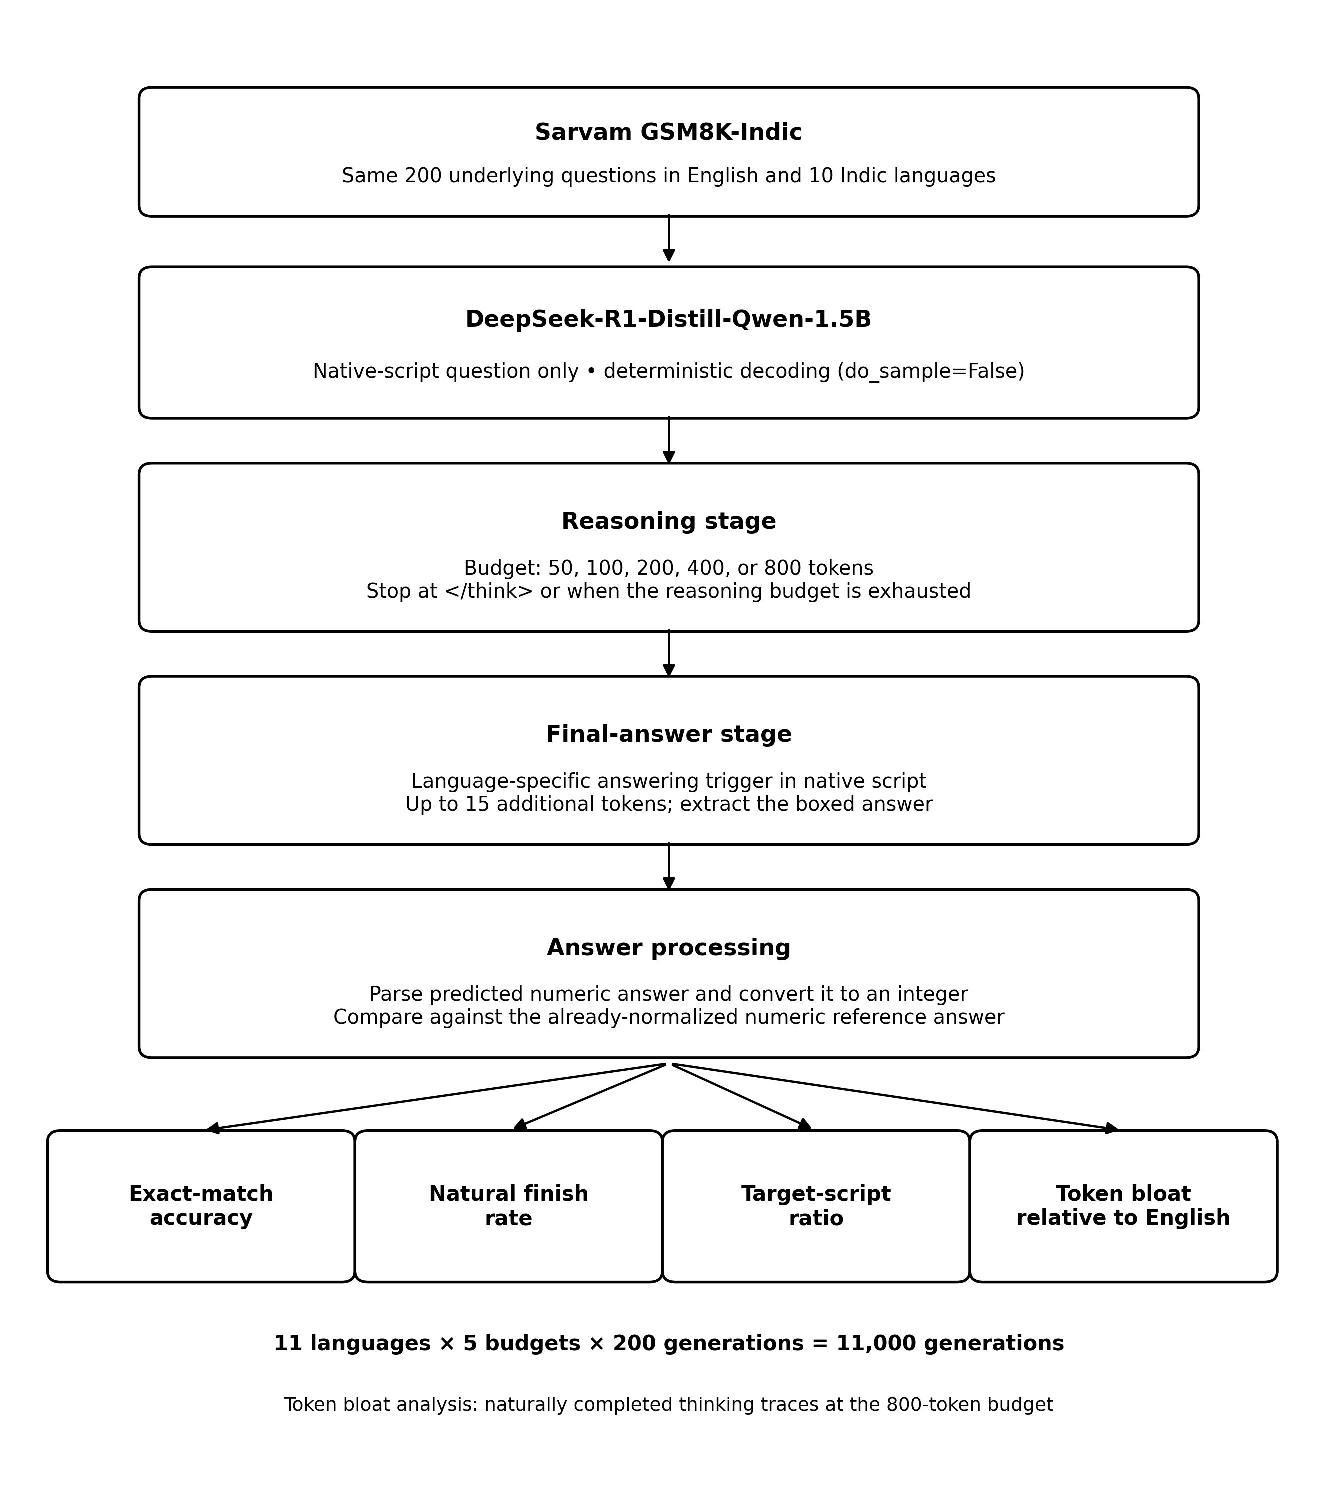
\includegraphics[width=0.75\linewidth]
    {figures/figure1_experimental_pipeline.pdf}
    \caption{Experimental pipeline for evaluating mathematical reasoning
    across English and ten Indic languages under five reasoning-token
    budgets. Each language-budget condition contains 200 generations.}
    \label{fig:experimental_pipeline}
\end{figure}


\subsection{Model and Generation Settings}
\label{sec:model_generation}

We evaluate DeepSeek-R1-Distill-Qwen-1.5B, a distilled reasoning model with 1.5 billion parameters \citep{deepseek2025r1}. The current evaluation focuses on this model to establish how constrained reasoning budgets affect mathematical reasoning across English and ten Indic languages. Evaluation of additional small language models is planned for the remaining semester.

We consider five reasoning-token budgets: 50, 100, 200, 400, and 800 tokens. For each language, we use the same 200 questions across all five budget conditions. This results in 1,000 generations per language and 11,000 generations across the eleven language conditions.

We use deterministic decoding with \texttt{do\_sample=False}. The token budget applies only to the reasoning stage, rather than the complete generation. During this stage, generation stops when the model produces the closing marker \texttt{</think>} or when the specified reasoning-token budget is exhausted. If the budget is exhausted first, the reasoning trace is treated as truncated.

After the reasoning stage, we append a language-specific final-answer trigger and allow up to 15 additional tokens for generating the final answer. We use the corresponding trigger for each language to support answer extraction across the English and Indic-language conditions. These additional tokens are excluded from the reasoning-token budget.

Figure~\ref{fig:experimental_pipeline} summarizes the generation and evaluation procedure. This setup allows us to examine mathematical accuracy and reasoning completion under different token budgets while keeping the evaluated questions and decoding strategy consistent across budget conditions.



\subsection{Evaluation Metrics}
\label{sec:eval_metrics}

We evaluate mathematical reasoning under constrained token budgets using four metrics: exact-match accuracy, natural finish rate, character-level target-script ratio, and token bloat relative to English.

\textbf{Exact-Match Accuracy.}
We evaluate mathematical correctness by extracting the answer from the \texttt{\textbackslash boxed\{\}} expression generated after the language-specific answering trigger and comparing it with the reference answer. For each language and reasoning-token budget, accuracy is calculated over the 200 evaluated questions:

\begin{equation}
\text{Accuracy} =
\frac{\text{Number of correct answers}}
{\text{Number of evaluated questions}}
\times 100.
\end{equation}

This metric measures how mathematical accuracy changes as the available reasoning-token budget increases. Figure~\ref{fig:accuracy_budget} will compare accuracy across all eleven language conditions and five budgets.

\textbf{Natural Finish Rate.}
We measure the natural finish rate to determine how often the model completes its reasoning within the allocated token budget. A generation is classified as a natural finish when the model produces the \texttt{</think>} closing marker before the reasoning-token budget is exhausted. If the budget is exhausted first, the reasoning trace is classified as truncated.

The natural finish rate is calculated as:

\begin{equation}
\text{Finish Rate} =
\frac{\text{Number of natural finishes}}
{\text{Total number of generations}}
\times 100.
\end{equation}

This metric helps distinguish completed reasoning traces from those interrupted by the token limit. Figure~\ref{fig:completion_budget} will show how the natural finish rate changes across languages and budgets.

\textbf{Character-Level Target-Script Ratio.}
We measure the proportion of counted characters in a generated thinking trace that belong to the target language's script. Digits, whitespace, and punctuation are excluded. For language $\ell$, the ratio is defined as:

\begin{equation}
R_{\ell} =
\frac{C_{\ell}}{C_{\mathrm{counted}}}
\times 100,
\end{equation}

where $C_{\ell}$ is the number of counted characters belonging to the target script and $C_{\mathrm{counted}}$ is the total number of counted characters after excluding digits, whitespace, and punctuation. This metric measures script composition rather than semantic language choice or the number of language switches.

Figure~\ref{fig:script_ratio} will summarize target-script usage across languages. Figure~\ref{fig:script_accuracy} will examine the relationship between target-script ratio and mathematical accuracy.

\textbf{Token Bloat Relative to English.}
We measure token bloat as the ratio between the number of tokens in an Indic-language thinking trace and the number of tokens in the English thinking trace for the same underlying question. We restrict this comparison to paired traces that finish naturally at the 800-token reasoning budget. For language $\ell$ and question $i$, the multiplier is

\begin{equation}
B_{\ell,i} = \frac{T_{\ell,i}}{T_{\mathrm{en},i}}, \qquad
\overline{B}_{\ell} = \frac{1}{N_{\ell}}\sum_{i=1}^{N_{\ell}} B_{\ell,i},
\label{eq:token_bloat}
\end{equation}

where $T_{\ell,i}$ and $T_{\mathrm{en},i}$ are the numbers of thinking tokens for the Indic-language and English traces, respectively, and $N_{\ell}$ is the number of valid paired comparisons for language $\ell$. A value above $1$ indicates that the Indic-language trace used more tokens than its English counterpart. Figure~\ref{fig:token_bloat} and Table~\ref{tab:token_bloat} report the measured multipliers and comparison counts.



\subsection{Experimental Conditions and Comparison Strategy}
\label{sec:comparison_strategy}

We vary two experimental factors: language and reasoning-token budget. The language conditions comprise English and ten Indic languages, while the reasoning-token budgets are 50, 100, 200, 400, and 800 tokens. We evaluate all conditions using DeepSeek-R1-Distill-Qwen-1.5B.

We use the same 200 underlying GSM8K questions across all eleven languages. Each question is evaluated using its corresponding language version from the Sarvam GSM8K-Indic dataset. Within each language, the same 200 questions are reused across all five budget conditions. This design controls the evaluated question set when comparing results across languages and budgets.

Each language-budget condition contains 200 generations, resulting in 1,000 generations per language and 11,000 generations overall. English serves as the reference condition for comparisons with the Indic languages.

We compare exact-match accuracy and natural finish rate across token budgets to investigate how reasoning constraints affect answer correctness and completion. We also examine token bloat and target-script ratio to explore their relationships with mathematical accuracy and reasoning completion. Figure~\ref{fig:experimental_pipeline} summarizes the experimental workflow and evaluation stages.

The current comparison uses a single model. Therefore, the findings establish an initial evaluation of language-related differences under constrained reasoning budgets. Evaluating additional small language models is planned for the remainder of the semester.


\subsection{Implementation Details}
\label{sec:implementation}

We run the experiments locally on a personal computing device with a GPU that has 16 GB of memory. We load DeepSeek-R1-Distill-Qwen-1.5B using the Hugging Face Transformers interface, \texttt{AutoModelForCausalLM}. We use deterministic decoding with \texttt{do\_sample=False}.

For each language, the model receives the mathematical question in its native script without an additional instruction prompt. We evaluate the same 200 underlying questions across English and all ten Indic languages. Each language is evaluated under five reasoning-token budgets: 50, 100, 200, 400, and 800 tokens.

The reasoning stage terminates when the model generates the \texttt{</think>} closing marker or exhausts the allocated token budget. We classify the generation as a natural finish if the closing marker appears within the budget. Otherwise, we classify the reasoning trace as truncated. After this stage, we provide a language-specific answering trigger in the corresponding script and allow up to 15 additional tokens for the final answer. These additional tokens are not included in the reasoning-token budget.


We extract the predicted answer from the \texttt{\textbackslash boxed\{\}}
expression generated after the language-specific answering trigger. The
numeric parser removes dollar signs and commas, extracts numeric
substrings, and selects the first number found. We convert the parsed
prediction to an integer and compare it with the dataset's already-normalized
numeric reference answer. A prediction is counted as correct when the
integer values match.


The complete evaluation comprises 11,000 generations across eleven language conditions and five token-budget settings. We calculate exact-match accuracy, natural finish rate, character-level target-script ratio, and token bloat relative to English from the generated outputs. Figure~\ref{fig:experimental_pipeline} will summarize the complete experimental workflow.


% ---------------------------------------------------------------
% 5. RESULTS AND DISCUSSION
% ---------------------------------------------------------------
% Instructions:
%   - One sub-section per experiment / research question.
%   - Each sub-section: (1) state the objective, (2) present a table or
%     figure, (3) discuss findings with intuition and explanation.
%   - Every table and figure must have a caption and be discussed in text.
%   - Best results in \textbf{bold}; second-best \underline{underlined}.
%   - Use $\dagger$ to mark statistically significant results.
% ---------------------------------------------------------------




\section{Results and Discussion}
\label{sec:results}

\subsection{Effect of Reasoning-Token Budget on Mathematical Accuracy}

Figure~\ref{fig:accuracy_budget} shows the exact-match accuracy of DeepSeek-R1-Distill-Qwen-1.5B across English and ten Indic languages under five reasoning-token budgets. The evaluation uses the same 200 underlying mathematical questions across all languages and budgets.

English achieves the highest accuracy overall. Its accuracy increases from 21.0\% at the 50-token budget to 64.0\% at the 800-token budget. This represents an improvement of 43 percentage points as the available reasoning budget increases.

Among the Indic languages, Hindi achieves the highest accuracy in the reported results. Its accuracy rises from 5.5\% at 50 tokens to 24.0\% at 800 tokens. Bengali also improves across the evaluated budgets, increasing from 2.0\% to 9.5\%. These results indicate that additional reasoning tokens can improve mathematical accuracy, although the magnitude of the improvement differs across languages.

However, the relationship between budget size and accuracy is not uniformly increasing across the Indic languages. Some languages show limited gains or fluctuations as the budget increases. For example, the reported accuracy for Gujarati changes from 6.0\% at 50 tokens to 6.5\% at 800 tokens, while Malayalam remains within a relatively narrow range across the five conditions. Such patterns suggest that a larger token budget alone does not guarantee a comparable improvement in mathematical reasoning accuracy across languages.

The gap between English and the Indic languages remains substantial even at the largest evaluated budget. Hindi, the strongest Indic-language condition in the reported results, reaches 24.0\% accuracy at 800 tokens, compared with 64.0\% for English. This difference motivates further investigation into whether tokenization differences, reasoning completion, and target-script usage are associated with the observed performance gap.

Overall, the results show that reasoning-token budgets affect mathematical accuracy, but their effects differ across languages. The accuracy curves provide the first part of the analysis. The next subsection examines natural finish rates to determine how often the model completes its reasoning within the available budget.

\begin{figure}[htbp]
    \centering
    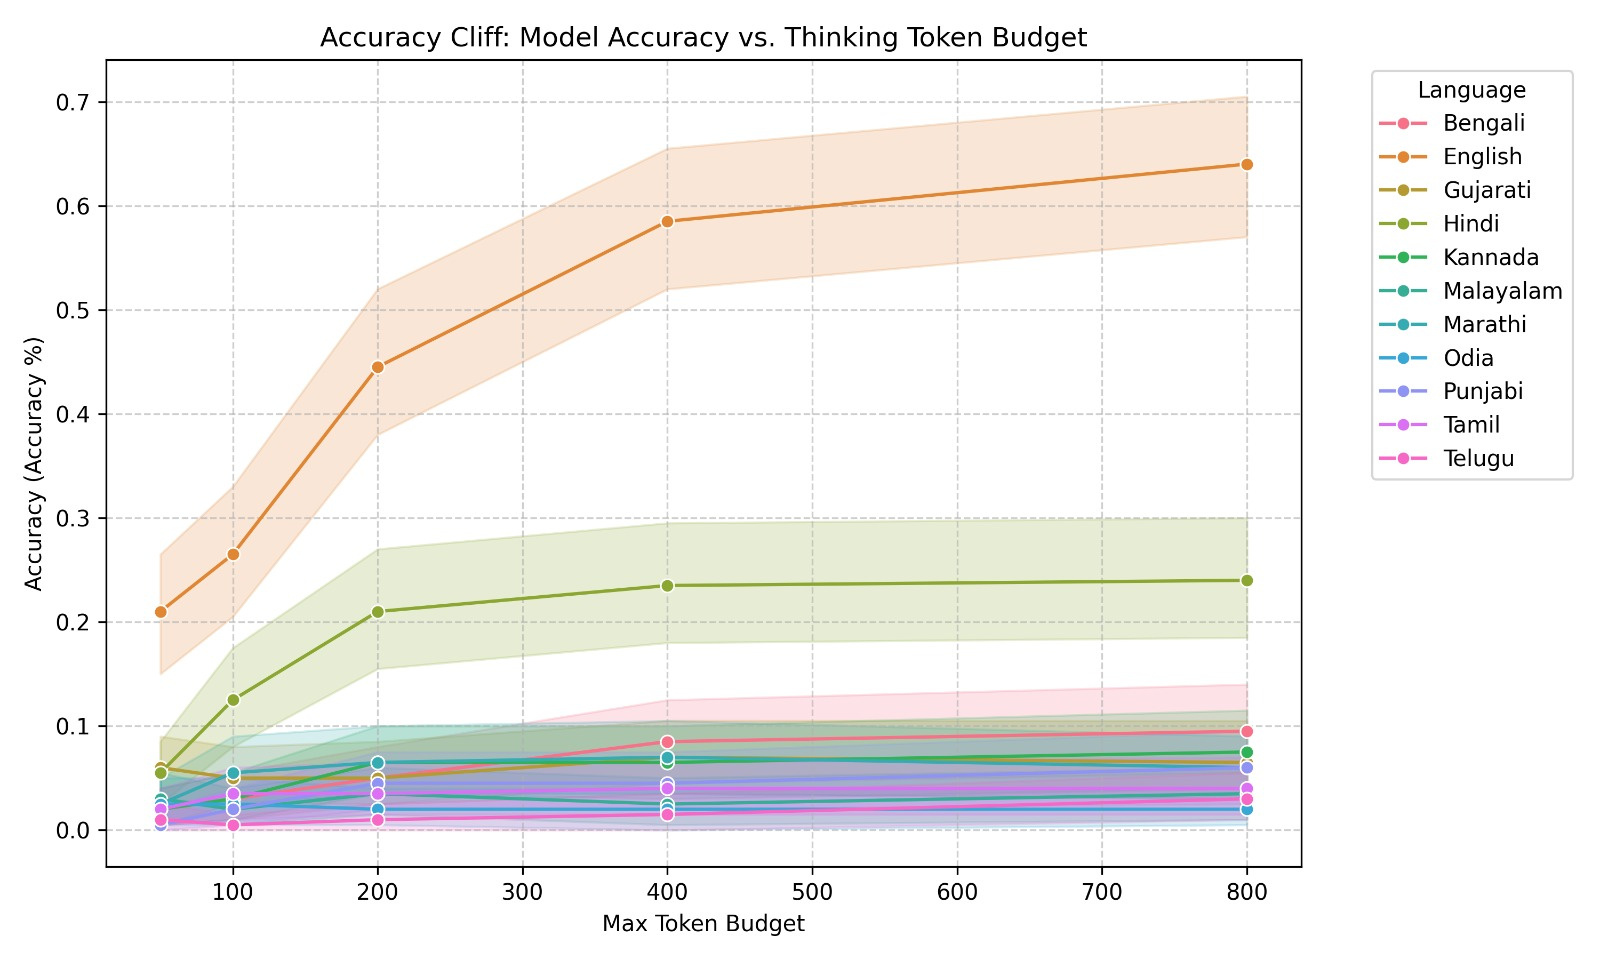
\includegraphics[width=\linewidth]
    {figures/accuracy_budget.jpg}
    \caption{Mathematical accuracy of DeepSeek-R1-Distill-Qwen-1.5B
    across English and ten Indic languages under five reasoning-token
    budgets. The same 200 underlying questions are evaluated at each
    budget for every language.}
    \label{fig:accuracy_budget}
\end{figure}


\subsection{Natural Finish Rate Under Token Budgets}
\label{subsec:natural_finish}

Figure~\ref{fig:completion_budget} shows the natural finish rate of DeepSeek-R1-Distill-Qwen-1.5B across English and ten Indic languages under the five reasoning-token budgets. A generation counts as a natural finish when the model produces the \texttt{</think>} closing marker before exhausting its allocated reasoning-token budget. Otherwise, the reasoning trace is classified as truncated.

The natural finish rate generally increases with the available token budget across most language conditions. Smaller budgets frequently interrupt reasoning before the model produces the closing marker. Larger budgets provide more room for the model to complete its reasoning trace, reducing the proportion of budget-induced cutoffs.

However, the completion patterns differ across languages. Gujarati shows a notably lower natural finish rate than most other language conditions, even as the available budget increases. This suggests that increasing the token budget alone does not eliminate the differences in reasoning completion across languages. The results motivate further investigation into whether differences in token bloat and target-script usage are associated with these completion patterns.

Natural finish rate and mathematical accuracy capture different aspects of model behavior. A trace may terminate naturally but still contain incorrect reasoning or an incorrect final answer. Conversely, a trace interrupted by the token limit may already contain enough information to produce the correct answer. We therefore interpret completion rates alongside the accuracy results rather than treating natural completion as evidence of correctness.

Overall, these results show that larger reasoning-token budgets generally allow more traces to finish naturally, but the extent of this improvement varies across languages. The next subsection examines token bloat relative to English to investigate whether relative token use is associated with these completion differences.


\begin{figure}[htbp]
    \centering
    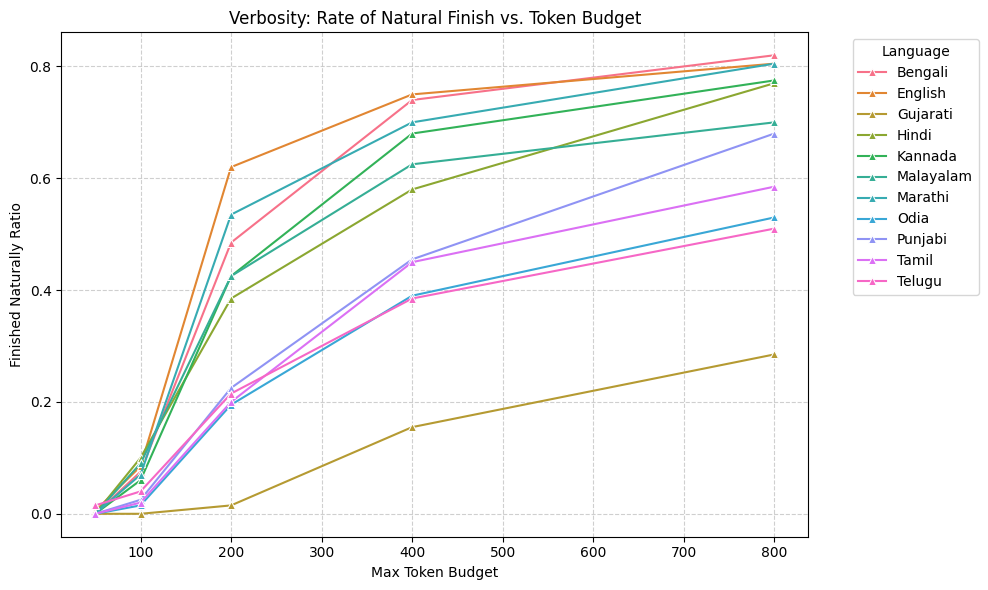
\includegraphics[
        width=\linewidth,
        keepaspectratio
    ]{figures/completion_budget.jpg}
    \caption{Natural finish rate of DeepSeek-R1-Distill-Qwen-1.5B
    across English and ten Indic languages under five reasoning-token
    budgets. A natural finish occurs when the model generates the
    \texttt{</think>} marker before exhausting the reasoning-token budget.}
    \label{fig:completion_budget}
\end{figure}


\subsection{Token Bloat Across Languages}

We measure token bloat relative to English to examine differences in token usage across languages. The analysis considers generations produced under the 800-token reasoning budget that finished their thinking stage naturally. For each Indic language, we compare valid question pairs against the English condition and calculate the average token bloat multiplier. Table~\ref{tab:token_bloat} reports the number of valid comparisons and the average multiplier for each language.

Gujarati exhibits the highest token bloat multiplier at 2.85$\times$ relative to English, based on 49 valid question comparisons. Punjabi follows at 2.46$\times$, while Telugu and Odia show multipliers of 2.17$\times$ and 2.04$\times$, respectively. Tamil has a multiplier of 2.02$\times$, and Hindi has a multiplier of 1.87$\times$. Bengali and Kannada exhibit multipliers of 1.74$\times$ and 1.72$\times$, respectively. Malayalam and Marathi have the lowest multipliers, at 1.59$\times$ and 1.54$\times$.

These results indicate substantial differences in token usage across the evaluated languages. In the analyzed question pairs, generated thinking traces in every Indic language have a higher average token count than their English counterparts. The size of this difference varies across languages, with Gujarati showing the largest relative token cost and Marathi the smallest.

The Gujarati result is particularly noteworthy when considered alongside the completion analysis in Section~\ref{subsec:natural_finish}. Gujarati has the highest measured token bloat multiplier and a notably low natural finish rate. One possible explanation is that greater token consumption leaves less room for completing a reasoning trace within a fixed budget. However, the current observations do not establish that token bloat causes premature cutoffs. Language-specific reasoning behavior and differences in the valid comparison sets may also contribute to the observed pattern.

The valid comparison counts differ across languages, ranging from 49 for Gujarati to 138 for Bengali. Therefore, the reported averages are based on different numbers of question pairs. In particular, the Gujarati estimate should be interpreted with caution because it is based on fewer valid comparisons. Further analysis across matched examples and additional models will help determine whether the observed differences persist.

Overall, the results provide evidence of a language-dependent token cost under the evaluated generation conditions. This finding motivates further investigation into how tokenization and reasoning behavior interact under constrained budgets.


\begin{figure}[htbp]
    \centering
    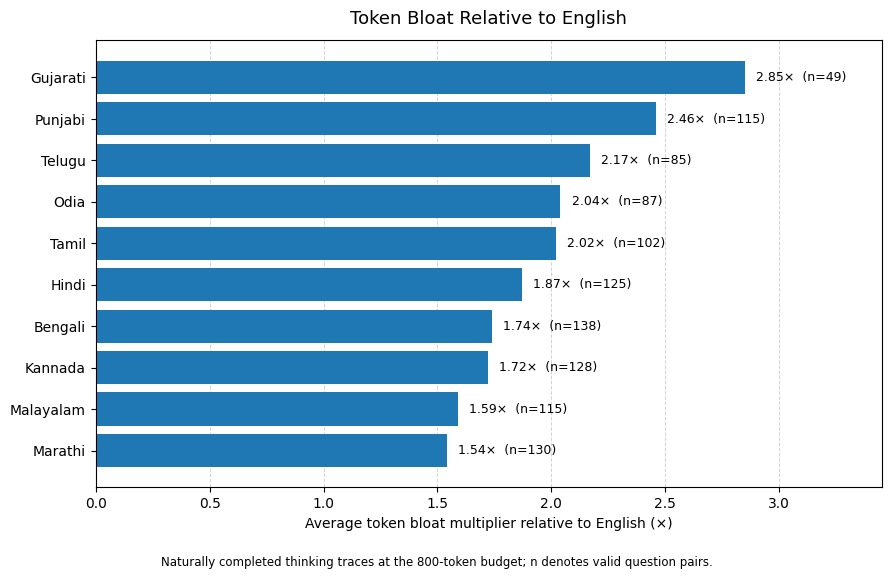
\includegraphics[width=0.95\linewidth]
    {figures/token_bloat.jpg}
    \caption{Average token bloat multiplier relative to English for
    naturally completed thinking traces under the 800-token reasoning
    budget. The values show the average multiplier for each language,
    with the number of valid question pairs indicated beside each bar.}
    \label{fig:token_bloat}
\end{figure}



\begin{table}[t]
\centering
\small
\setlength{\tabcolsep}{4pt}
\renewcommand{\arraystretch}{1.12}
\caption{Token bloat relative to English for naturally completed
thinking traces under the 800-token reasoning budget.}
\label{tab:token_bloat}
\begin{tabular}{@{}lrr@{}}
\toprule
Language & Valid pairs & Bloat ($\times$) \\
\midrule
Gujarati  & 49  & 2.85 \\
Punjabi   & 115 & 2.46 \\
Telugu    & 85  & 2.17 \\
Odia      & 87  & 2.04 \\
Tamil     & 102 & 2.02 \\
Hindi     & 125 & 1.87 \\
Bengali   & 138 & 1.74 \\
Kannada   & 128 & 1.72 \\
Malayalam & 115 & 1.59 \\
Marathi   & 130 & 1.54 \\
\bottomrule
\end{tabular}
\end{table}

\subsection{Target-Script Usage and Mathematical Accuracy}

We examine the relationship between target-script usage and mathematical accuracy to investigate whether generating reasoning in an Indic language's native script is associated with better performance. We use the character-level target-script ratio defined in Section~\ref{sec:eval_metrics} and compare it with exact-match accuracy across languages.

Gujarati exhibits the highest target-script usage among the evaluated Indic languages. Its reasoning traces retain substantially more of the target script than those of the other Indic-language conditions. However, Gujarati also exhibits a low natural finish rate and the highest token bloat multiplier relative to English in our 800-token analysis. These findings show that greater target-script usage can coexist with a higher token cost and more frequent reasoning truncation.

Hindi provides a useful contrast. It achieves the highest mathematical accuracy among the Indic languages, although Gujarati shows stronger target-script persistence. This difference suggests that native-script usage alone does not explain the observed accuracy ranking. Other factors, including tokenization cost and language-specific model behavior, may also contribute to performance differences.

We further examine accuracy across groups of reasoning traces with different target-script ratios. Figure~\ref{fig:script_accuracy} will present this comparison, while Figure~\ref{fig:script_ratio} will summarize target-script usage across languages. These analyses help assess whether traces with greater target-script usage tend to achieve higher accuracy within each language.

The target-script ratio measures the proportion of counted characters belonging to the target writing system. It does not directly identify semantic language choice or count switches between languages. Therefore, we interpret this metric as a measure of script composition rather than a direct measure of language switching.

Taken together, the results do not support treating native-script persistence as a sufficient indicator of mathematical reasoning quality. Gujarati's high target-script usage alongside its low finish rate and high token bloat highlights the need to study script composition, tokenization cost, reasoning completion, and accuracy together. These observed relationships are descriptive and do not establish that using a native script causes either higher or lower mathematical accuracy.

\begin{figure}[htbp]
    \centering
    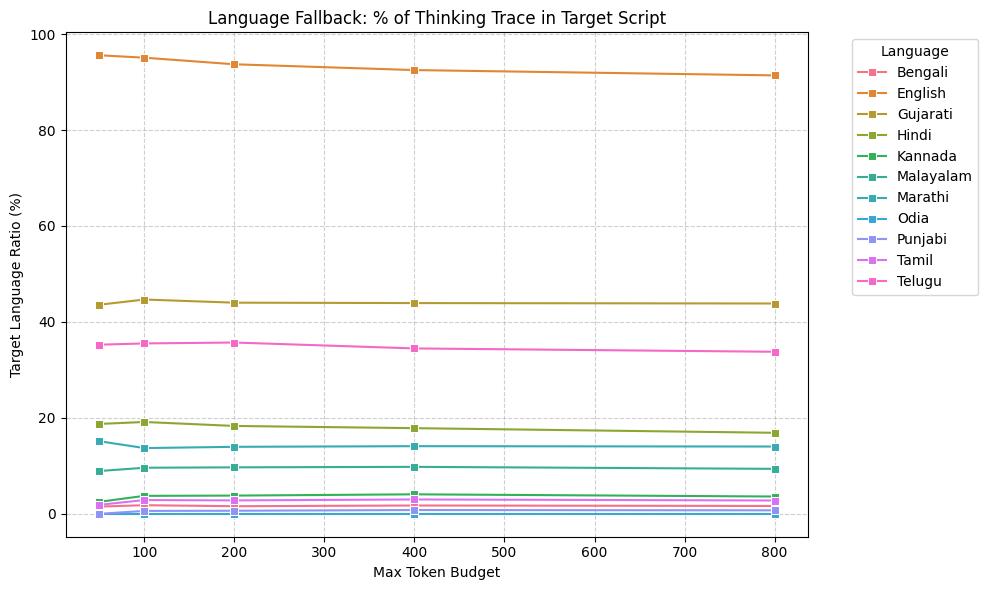
\includegraphics[width=0.95\linewidth]
    {figures/script_ratio.jpg}
    \caption{Percentage of each language's thinking trace written in
    its target script across five reasoning-token budgets, for English
    and ten Indic languages.}
    \label{fig:script_ratio}
\end{figure}


\begin{figure}[htbp]
    \centering
    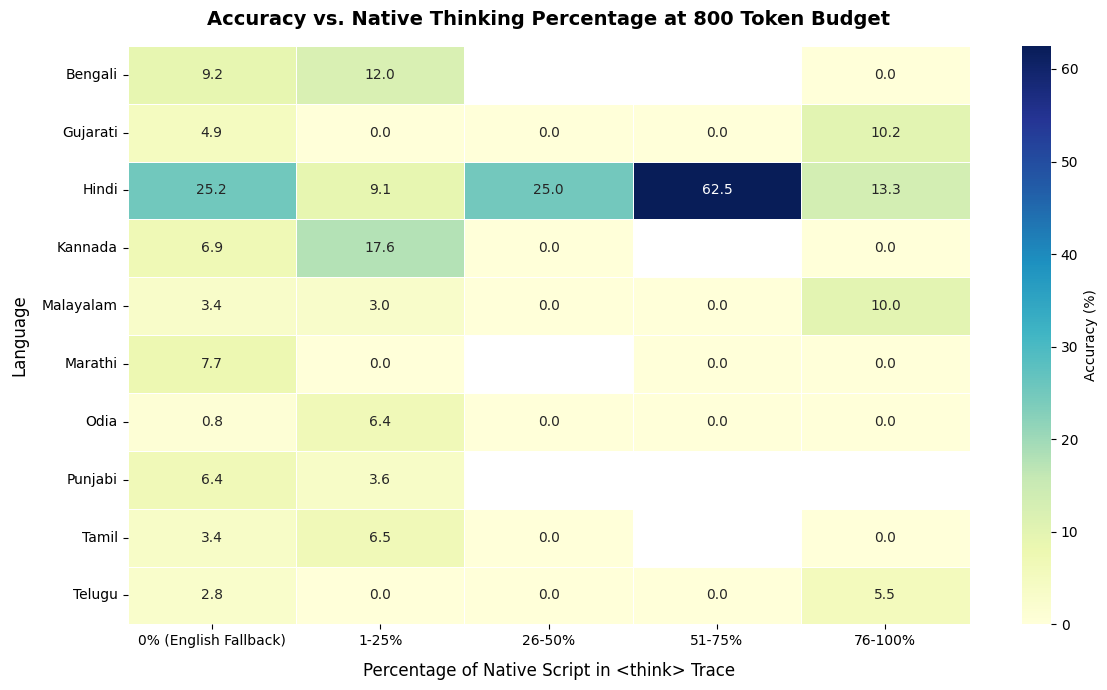
\includegraphics[width=\linewidth]
    {figures/figure6_script_accuracy_heatmap.jpg}
    \caption{Exact-match accuracy grouped by target-script ratio for
    English fallback and native-script reasoning traces at the
    800-token reasoning budget. Blank cells indicate groups for which
    no value is displayed in the supplied results.}
    \label{fig:script_accuracy}
\end{figure}


\subsection{Overall Discussion}

The experiments reveal differences in mathematical reasoning accuracy, reasoning completion, token usage, and target-script persistence across English and ten Indic languages. These results provide an initial view of how reasoning-token constraints affect DeepSeek-R1-Distill-Qwen-1.5B across languages.

\textbf{RQ1: Effect of reasoning-token budgets.}
English achieves the highest mathematical accuracy across the evaluated conditions. Among the Indic languages, Hindi achieves the highest accuracy. Although larger reasoning budgets improve accuracy in several languages, the gains vary across languages, and some show limited improvement as the budget increases. This suggests that increasing the available reasoning tokens does not produce uniform improvements across language conditions.

\textbf{RQ2: Relationship between token usage and reasoning completion.}
The token bloat analysis shows that all ten Indic languages require more tokens than English for the compared, naturally completed thinking traces. Gujarati has the highest average token bloat multiplier at 2.85$\times$, while Marathi has the lowest at 1.54$\times$. Gujarati also exhibits a notably low natural finish rate. These observations are consistent with the possibility that higher token consumption leaves less room for reasoning under a fixed budget. However, the current results establish an association rather than a causal relationship.

\textbf{RQ3: Target-script persistence and accuracy.}
Gujarati exhibits the strongest target-script persistence among the evaluated Indic languages, but Hindi achieves higher mathematical accuracy. This indicates that greater native-script usage does not necessarily correspond to better mathematical reasoning performance. Script composition, token consumption, and reasoning completion capture different aspects of generation and should be examined together.

Taken together, the results show that the effect of a fixed reasoning-token budget differs across language conditions. The observed differences motivate further investigation into how tokenization cost and language-specific generation behavior contribute to mathematical reasoning performance. Since the current experiments evaluate one model, additional model evaluations are required before determining whether these patterns extend to other small language models.

\subsection{Research Progress and Planned Evaluation}
The current stage includes the completed evaluation of DeepSeek-R1-Distill-Qwen-1.5B across English and ten Indic languages under five reasoning-token budgets. The analysis covers exact-match accuracy, natural finish rate, character-level target-script ratio, and token bloat relative to English.

The remaining work includes evaluating additional small language models, comparing language-specific trends across models, and refining the analysis of token usage and reasoning completion. We will also validate the consistency of the evaluation pipeline, consolidate the experimental results, and prepare the final figures and tables.

These additional experiments will help determine whether the observed language differences are specific to the current model or recur across different model sizes and architectures.

% ---------------------------------------------------------------
% 6. CONCLUSION
% ---------------------------------------------------------------
% Instructions:
%   - 2-3 paragraphs; a refined, forward-looking version of the abstract.
%   - Be specific: mention actual numbers, dataset names, method names.
%   - Do NOT simply copy-paste the abstract.
% ---------------------------------------------------------------

\section{Conclusion}

This study investigates whether fixed reasoning-token budgets affect mathematical reasoning differently across English and ten Indic languages. We evaluate DeepSeek-R1-Distill-Qwen-1.5B on the Sarvam GSM8K-Indic dataset using five reasoning-token budgets, from 50 to 800 tokens. Our analysis considers mathematical accuracy, natural finish rate, target-script usage, and token bloat relative to English.

The results reveal substantial differences across language conditions. English achieves the highest mathematical accuracy, while Hindi performs best among the evaluated Indic languages. Increasing the reasoning-token budget improves accuracy in several languages, but the magnitude of improvement varies. A larger budget therefore does not guarantee uniform gains across languages.

Our token bloat analysis identifies additional differences in token usage. Among the evaluated Indic languages, Gujarati has the highest average token bloat multiplier relative to English, at 2.85$\times$, while Marathi has the lowest, at 1.54$\times$, for the naturally completed thinking traces analyzed under the 800-token budget. Gujarati also exhibits a notably low natural finish rate despite having the strongest target-script persistence among the Indic languages. In contrast, Hindi achieves the highest Indic-language accuracy. These findings show that target-script usage, token consumption, reasoning completion, and mathematical accuracy do not necessarily follow the same pattern.

Overall, the findings provide initial evidence that a shared reasoning-token budget can lead to different generation and accuracy outcomes across languages. Token bloat is a plausible contributor to these differences, but the current results do not establish a causal relationship between tokenization cost and mathematical accuracy. The findings also come from a single model and should not yet be generalized to all small language models.

Future work will evaluate additional small language models to determine whether these patterns persist across model sizes and architectures. We will also refine cross-language comparisons and further examine the relationship between token bloat, reasoning completion, target-script usage, and answer accuracy. This broader evaluation will help establish whether token-budget policies require language-sensitive considerations when applied to multilingual reasoning systems.

% \bibliographystyle{acl_natbib}
\bibliography{custom}

\end{document}


% \documentclass[11pt]{article}

% % Change "review" to "final" to generate the final (sometimes called camera-ready) version.
% % Change to "preprint" to generate a non-anonymous version with page numbers.
% \usepackage[review]{acl}
% \usepackage{float}
% % Standard package includes
% \usepackage{times}
% \usepackage{latexsym}
% \usepackage{graphicx}
% % For proper rendering and hyphenation of words containing Latin characters (including in bib files)
% \usepackage[T1]{fontenc}
% % For Vietnamese characters
% % \usepackage[T5]{fontenc}
% % See https://www.latex-project.org/help/documentation/encguide.pdf for other character sets

% % This assumes your files are encoded as UTF8
% \usepackage[utf8]{inputenc}

% % This is not strictly necessary, and may be commented out,
% % but it will improve the layout of the manuscript,
% % and will typically save some space.
% \usepackage{microtype}

% % This is also not strictly necessary, and may be commented out.
% % However, it will improve the aesthetics of text in
% % the typewriter font.
% \usepackage{inconsolata}

% % Including images in your LaTeX document requires adding
% % additional package(s)
% \usepackage{graphicx}

% % Additional packages for the skeleton
% \usepackage{booktabs}       % professional tables (\toprule, \midrule, \bottomrule)
% \usepackage{multirow}       % multi-row table cells
% \usepackage{tabularx}       % flexible-width tables
% \usepackage{amsmath}        % math environments
% \usepackage{amssymb}        % math symbols
% \usepackage{xcolor}         % colored text for TODO notes
% \usepackage{enumitem}       % customise list spacing

% % If the title and author information does not fit in the area allocated, uncomment the following
% %
% %\setlength\titlebox{<dim>}
% %
% % and set <dim> to something 5cm or larger.

% % ---------------------------------------------------------------
% % Useful commands for filling in the skeleton
% % ---------------------------------------------------------------
% \newcommand{\eg}{\textit{e.g.,}\ }
% \newcommand{\ie}{\textit{i.e.,}\ }
% \newcommand{\etal}{\textit{et al.}}
% % Use \TODO{} to mark sections that still need content (shows in red)
% \newcommand{\TODO}[1]{\textcolor{red}{\textbf{[TODO: #1]}}}
% % Use \NOTE{} to leave yourself internal notes (shows in blue)
% \newcommand{\NOTE}[1]{\textcolor{blue}{\textit{[NOTE: #1]}}}

% % ---------------------------------------------------------------
% % TITLE
% % ---------------------------------------------------------------
% \title{[Your Paper Title Here: Concise, Descriptive, and Keyword-Rich]}

% % ---------------------------------------------------------------
% % AUTHORS
% % ---------------------------------------------------------------
% % For several authors from the same institution:
% % \author{Author 1 \and ... \and Author n \\
% %         Address line \\ ... \\ Address line}
% % if the names do not fit well on one line use
% %         Author 1 \\ {\bf Author 2} \\ ... \\ {\bf Author n} \\
% % For authors from different institutions:
% % \author{Author 1 \\ Address line \\  ... \\ Address line
% %         \And  ... \And
% %         Author n \\ Address line \\ ... \\ Address line}
% % To start a separate ``row'' of authors use \AND, as in
% % \author{Author 1 \\ Address line \\  ... \\ Address line
% %         \AND
% %         Author 2 \\ Address line \\ ... \\ Address line \And
% %         Author 3 \\ Address line \\ ... \\ Address line}

% \author{First Author \\
%   Affiliation / Address line 1 \\
%   Affiliation / Address line 2 \\
%   Affiliation / Address line 3 \\
%   \texttt{email@domain} \\\And
%   Second Author \\
%   Affiliation / Address line 1 \\
%   Affiliation / Address line 2 \\
%   Affiliation / Address line 3 \\
%   \texttt{email@domain} \\}

% %\author{
% %  \textbf{First Author\textsuperscript{1}},
% %  \textbf{Second Author\textsuperscript{1,2}},
% %  \textbf{Third T. Author\textsuperscript{1}},
% %  \textbf{Fourth Author\textsuperscript{1}},
% %\\
% %  \textbf{Fifth Author\textsuperscript{1,2}},
% %  \textbf{Sixth Author\textsuperscript{1}},
% %  ...
% %\\
% %  \textsuperscript{1}Affiliation 1,
% %  \textsuperscript{2}Affiliation 2
% %\\
% %  \small{
% %    \textbf{Correspondence:} \href{mailto:email@domain}{email@domain}
% %  }
% %}

% % ===============================================================
% \begin{document}
% \maketitle
% % ===============================================================

% % ---------------------------------------------------------------
% % ABSTRACT
% % ---------------------------------------------------------------
% % Instructions: 150-250 words. No citations. Cover four points:
% %   (1) Problem statement  (2) Research gap
% %   (3) Approach           (4) Key experimental result
% % ---------------------------------------------------------------
% \begin{abstract}
% Recent efficiency methods train large language models to reduce reasoning length to save computational resources. Prior research documents tokenizer inefficiencies but fails to audit how strict token budgets cap the reasoning capabilities of Indic languages. We investigate this problem by analyzing cross-lingual reasoning degradation under constrained budgets. We use a character-level script tracking metric to separate tokenizer bloat from true logical deficits. We evaluate reasoning on various math problem sets, starting with a translated GSM8K benchmark across ten Indic languages. We test multiple reasoning models, beginning with a distilled lightweight model, across five strict token budgets. High token fertility causes a severe reasoning cliff and forces premature generation cutoffs. Surprisingly, most evaluated languages achieve peak mathematical accuracy when the model successfully sustains native script reasoning instead of completely falling back to English. These findings emphasize the need for content-based reasoning budgets to prevent the systematic degradation of non-English capabilities.
% \end{abstract}
% % ---------------------------------------------------------------
% % 1. INTRODUCTION
% % ---------------------------------------------------------------
% \section{Introduction}
% \label{sec:intro}

% Large language models (LLMs) are increasingly used for tasks that require mathematical and logical reasoning. These models can generate intermediate reasoning steps before producing a final answer \citep{wei2022chain, openai2024o1}. However, their performance can vary across languages. Previous evaluations have reported differences between English and non-English reasoning performance \citep{shi2022language, longcot2025}. These differences raise questions about whether LLMs provide comparable reasoning capabilities across linguistic populations.

% Recent methods aim to reduce the computational cost of reasoning by controlling the length of generated responses \citep{aggarwal2025l1, hou2025thinkprune}. These methods often impose a maximum number of generated tokens, known as a token budget. The effects of a fixed budget may vary across languages because tokenizers can represent equivalent content using different numbers of tokens. Studies have reported inefficiencies in tokenization for non-Latin scripts, including Indic scripts \citep{tokenizertax2026, brahmic2026}. Consequently, a mathematical problem may require a longer generated sequence in one language than in another. When the available budget is insufficient, a model may stop generating before completing its reasoning or producing a final answer. This raises the question of how tokenization and generation limits affect mathematical reasoning across languages.

% Prior research has examined methods for reducing reasoning length and controlling the number of generated tokens \citep{liu2025laser, shorterbetter2025}. Other studies have investigated multilingual reasoning performance and the representation of Indic languages by existing tokenizers \citep{crosslingual2025, indicparam2025}. Recent work has also examined the relationship between output-token budgets and multilingual reasoning performance \citep{mindthecap2026}. Research on language switching during reasoning provides further context for understanding the role of English in multilingual model outputs \citep{mcd2026}. However, the relationship between token budgets, target-script usage, generation completion, and mathematical accuracy across Indic languages requires further investigation. In particular, it remains necessary to examine whether script usage is associated with reasoning performance under different generation limits.

% We investigate these questions by evaluating mathematical reasoning across eight Indic languages and English. We use translated versions of the GSM8K mathematical reasoning benchmark \citep{cobbe2021gsm8k} and evaluate the DeepSeek-R1-Distill-Qwen-1.5B model \citep{deepseek2025r1}. We consider five token budgets of 50, 100, 200, 400, and 800 tokens. At each budget, we measure exact-match answer accuracy and whether the generated reasoning finishes naturally or reaches the imposed limit. We also analyze target-script usage through a character-level metric that estimates the proportion of generated reasoning characters belonging to the target script. This analysis allows us to examine how script usage and generation completion vary across languages and token budgets.

% Our experiments show that mathematical accuracy and natural completion rates generally improve as the token budget increases, although the size of the improvement varies across languages. For example, from the smallest to the largest budget, English accuracy increases from 21\% to 64\%, while Hindi accuracy increases from 5.5\% to 24\%. The relationship between script usage and accuracy also varies by language. Aggregate results show higher accuracy for native-script reasoning traces in Bengali, Gujarati, Kannada, and Malayalam. English-thinking traces achieve higher aggregate accuracy in Hindi, Marathi, Odia, and Punjabi. These findings indicate that script usage alone does not predict mathematical reasoning accuracy consistently across languages. They also motivate further investigation into language-sensitive evaluation methods that account for tokenization differences and generation limits.

% \paragraph{Contributions.}
% Our main contributions are as follows.
% \begin{itemize}
%     \item \textbf{Budget-Based Multilingual Evaluation:} We evaluate mathematical reasoning accuracy and natural generation completion across five token budgets for eight Indic languages and English.

%     \item \textbf{Character-Level Script Analysis:} We measure target-script usage in generated reasoning traces and examine its relationship with mathematical accuracy across languages and token budgets.

%     \item \textbf{Analysis of Language-Specific Performance:} We characterize how token budgets, script usage, and generation completion relate to mathematical reasoning accuracy, identifying differences across the evaluated languages.

%     \item \textbf{Diagnostic Visualization Tools:} We provide interactive HTML dashboards for inspecting generated reasoning traces, script-usage measurements, and generation termination at the sample level.
% \end{itemize}
% % ---------------------------------------------------------------
% % 2. RELATED WORK
% % ---------------------------------------------------------------
% % Instructions:
% %   - 2-3 thematic sub-sections covering different categories of prior work.
% %   - Each sub-section: discuss 5-10 papers grouped by theme or approach.
% %   - END every sub-section with an explicit statement of how your work
% %     differs or what gap it fills. This is mandatory.
% % ---------------------------------------------------------------
% % ---------------------------------------------------------------
% % 2. RELATED WORK
% % ---------------------------------------------------------------
% \section{Related Work}
% \label{sec:related}

% \subsection{Efficient Reasoning and Length Constraints}
% \label{sec:related_cat1}

% Recent works train language models to reduce the length of reasoning traces. Researchers apply hard token caps during training or penalize long responses using reinforcement learning \citep{aggarwal2025l1, hou2025thinkprune}. Adaptive methods shape rewards based on sequence length and problem difficulty \citep{liu2025laser, shorterbetter2025}. Other methods enforce strict budget constraints during inference \citep{muennighoff2025s1}. These approaches successfully reduce computational costs. They primarily evaluate performance on English datasets. The underlying assumption across these works is that token count accurately reflects reasoning complexity. 

% \noindent\textbf{Gap addressed by this paper:}
% These efficiency methods assume that a token has equal semantic weight across all languages. We evaluate how these token-based budgets artificially suppress the reasoning capacity of Indic languages.

% \subsection{Multilingual Reasoning Capabilities}
% \label{sec:related_cat2}

% Language models exhibit significant performance drops when reasoning in non-English languages \citep{shi2022language, longcot2025}. Studies show that complex multi-step problems widen this cross-lingual gap. Researchers observe that reinforcement learning pushes models to abandon native scripts and fall back to English \citep{crosslingual2025}. Other methods attempt to compress multilingual chains of thought via cross-lingual distillation or native-language reinforcement learning \citep{mcd2026, ganitllm2026}. These studies document the fragility of non-English reasoning. They frequently attribute failures to poor language comprehension or limited training data.

% \noindent\textbf{Gap addressed by this paper:}
% Prior studies often assume that falling back to English inherently improves reasoning accuracy. We demonstrate that sustaining native script reasoning actually yields higher mathematical accuracy for several Indic languages.

% \subsection{Tokenizer Inefficiency and Sequence Bloat}
% \label{sec:related_cat3}

% Standard tokenizers struggle to encode non-Latin scripts efficiently. Studies document a severe tokenization penalty for Indic languages \citep{tokenizertax2026, brahmic2026}. A single mathematical thought in Malayalam or Tamil requires many more tokens than its English equivalent. Researchers benchmark low-resource Indic languages to highlight this structural inefficiency \citep{indicparam2025}. Recent evaluations also show how hidden token caps degrade performance in languages like German and Thai \citep{mindthecap2026}. These papers establish that non-English languages pay a higher computational cost.

% \noindent\textbf{Gap addressed by this paper:}
% Existing literature identifies token bloat but fails to connect it to forced efficiency methods. We isolate the tokenizer tax from true logical deficits by tracking exact native script ratios during strict budget cutoffs.

% % ---------------------------------------------------------------
% % 3. METHODOLOGY
% % ---------------------------------------------------------------
% % Instructions:
% %   - Describe WHAT you did at a conceptual level.
% %   - Do NOT include code-level details (no library names, function names,
% %     Python code, etc.).
% %   - Include a system/block diagram (Figure 1) --- MANDATORY.
% %     Use tools like Napkin AI, Excalidraw, or draw.io for a first draft.
% %   - The diagram should be colorful and visually appealing.
% % ---------------------------------------------------------------

% % ---------------------------------------------------------------
% % 3. METHODOLOGY
% % ---------------------------------------------------------------
% % ---------------------------------------------------------------
% % 3. METHODOLOGY
% % ---------------------------------------------------------------
% \section{Methodology}
% \label{sec:method}

% \subsection{Overview}
% \label{sec:method_overview}

% We evaluate mathematical reasoning under constrained generation budgets across ten Indic languages and English. Our experiments use the DeepSeek-R1-Distill-Qwen-1.5B model and GSM8K-derived mathematical reasoning datasets. For each question, the model generates an intermediate reasoning trace under a specified token budget. We then prompt the model to produce a final answer using a language-specific answer trigger. We assess mathematical accuracy and analyze reasoning completion and native-script usage across languages and budgets.

% \subsection{Dataset Selection}
% \label{sec:method_dataset}

% We use the GSM8K mathematical reasoning benchmark, which contains grade-school mathematical word problems that require multistep reasoning \citep{cobbe2021gsm8k}. We evaluate translated versions of the benchmark in ten Indic languages, namely Bengali, Gujarati, Hindi, Kannada, Malayalam, Marathi, Odia, Punjabi, Tamil, and Telugu. We also evaluate the original English benchmark as a reference for cross-lingual comparisons.

% Using translated versions of the same benchmark allows us to study how language variation affects reasoning performance on mathematically related problems. We retain the reference answer associated with each question to evaluate the model's final numerical prediction. This setup supports comparisons across languages while recognizing that translation differences may introduce variation in the linguistic presentation of a problem.

% \subsection{Budget-Constrained Reasoning Generation}
% \label{sec:method_generation}

% We evaluate the DeepSeek-R1-Distill-Qwen-1.5B model under five maximum generation budgets of 50, 100, 200, 400, and 800 tokens. Each question is evaluated separately at every budget. We use deterministic generation settings throughout the experiments.

% The model first generates a reasoning trace under the selected budget. If the trace contains the reasoning termination marker \texttt{</think>}, we retain the text preceding that marker and classify the trace as naturally completed. If the marker does not appear before the token limit is reached, we retain the generated trace and classify it as budget-truncated.

% This procedure allows us to distinguish traces that reach the model's reasoning termination marker from traces that exhaust their available generation budget. We record this completion status for each question, language, and budget combination.

% \subsection{Final Answer Generation and Evaluation}
% \label{sec:method_answer}

% After extracting the reasoning trace, we construct a continuation prompt that includes the original question, the retained reasoning text, and a language-specific final-answer trigger. The trigger follows the script and wording selected for the target language. For example, the English trigger is ``Final Answer:'', while the Hindi trigger is ``अंतिम उत्तर:''.

% We then allow the model to generate up to 15 additional tokens for the final answer. This separate stage applies the same answer-generation limit across the evaluated languages. It allows us to assess the answer produced after a reasoning trace has completed naturally or reached the imposed token budget.

% We extract the predicted numerical answer and compare it with the reference answer after normalizing formatting differences such as currency symbols and thousands separators. A prediction is counted as correct when the extracted numerical answer matches the reference answer. We calculate exact-match accuracy separately for each language and reasoning budget.

% \subsection{Character-Level Native Script Tracking}
% \label{sec:method_script}

% We analyze the character composition of each generated reasoning trace to measure the extent to which the model uses the target script. Let $C_{\text{native}}$ denote the number of characters assigned to the target script, and let $C_{\text{total}}$ denote the total number of characters in the retained reasoning trace.

% We define the native script ratio $R$ as

% \begin{equation}
%     R = \frac{|C_{\text{native}}|}{|C_{\text{total}}|} \times 100,
%     \label{eq:ratio}
% \end{equation}

% where $R$ represents the percentage of characters in the trace that belong to the target script. A higher value indicates greater use of that script, while a lower value indicates a larger proportion of characters outside it.

% We calculate this ratio for each reasoning trace and compare it across languages and token budgets. This analysis helps us examine the relationship between target-script usage, reasoning completion, and mathematical accuracy. The metric measures script composition and does not independently establish the language or meaning of every generated word.

% \subsection{Experimental Design}
% \label{sec:method_design}
% Our experimental design varies the maximum reasoning-trace budget while keeping the model and generation procedure fixed. We evaluate five budgets for each question and record the final-answer accuracy, reasoning completion status, and native script ratio.

% We analyze three outcomes. First, we measure how mathematical accuracy changes as the reasoning budget increases. Second, we examine the frequency of naturally completed and budget-truncated traces. Third, we investigate the relationship between native script ratios and final-answer accuracy across languages. Together, these analyses characterize how constrained reasoning generation relates to mathematical performance and script usage in Indic languages.
% % ---------------------------------------------------------------
% % 4. EXPERIMENTAL SETUP
% % ---------------------------------------------------------------
% % Instructions:
% %   - Use tables for datasets, models, metrics, and baselines.
% %   - Every dataset, model, metric, and baseline MUST be cited.
% %   - Follow the table formatting of the ACL template (hline or booktabs).
% % ---------------------------------------------------------------

% \section{Experimental Setup}

% \subsection{Dataset and Language Coverage}

% We use Sarvam AI's GSM8K-Indic dataset for our multilingual mathematical reasoning experiments \citep{sarvam_gsm8k_indic}. The dataset provides GSM8K mathematical problems in English and ten Indic languages: Bengali, Gujarati, Hindi, Kannada, Malayalam, Marathi, Odia, Punjabi, Tamil, and Telugu. These language versions allow us to investigate how language affects mathematical reasoning under constrained token budgets.

% Our evaluation covers eleven language conditions, including English as the reference condition. For each language, we select the same set of 200 questions and evaluate the model at five reasoning-token budgets: 50, 100, 200, 400, and 800 tokens. The same questions are reused across all five budgets within each language, enabling comparisons under different token constraints while keeping the question set fixed.

% Each language therefore contributes 1,000 generations, resulting in 11,000 generations across all eleven language conditions. This experimental design supports comparisons of mathematical accuracy and generation completion across languages and token budgets.

% As summarized in Figure~\ref{fig:figure1_experimental_pipeline}, the evaluation pipeline applies the selected token budget during reasoning generation and then evaluates the extracted final answer. We use exact-match accuracy, character-level target-script ratio, and token fertility to study answer correctness, script usage, and tokenization differences, respectively. The following subsections describe the model, generation procedure, and evaluation metrics in detail.

% \begin{figure}[H]
%     \centering
%     \includegraphics[width=0.75\linewidth]
%     {figures/figure1_experimental_pipeline.pdf}
%     \caption{Experimental pipeline for evaluating mathematical reasoning
%     across English and ten Indic languages under five reasoning-token
%     budgets. Each language-budget condition contains 200 generations.}
%     \label{fig:experimental_pipeline}
% \end{figure}


% \subsection{Model and Generation Settings}

% We evaluate DeepSeek-R1-Distill-Qwen-1.5B, a distilled reasoning model with 1.5 billion parameters \citep{deepseek2025r1}. The current evaluation focuses on this model to establish how constrained reasoning budgets affect mathematical reasoning across English and ten Indic languages. Evaluation of additional small language models is planned for the remaining semester.

% We consider five reasoning-token budgets: 50, 100, 200, 400, and 800 tokens. For each language, we use the same 200 questions across all five budget conditions. This results in 1,000 generations per language and 11,000 generations across the eleven language conditions.

% We use deterministic decoding with \texttt{do\_sample=False}. The token budget applies only to the reasoning stage, rather than the complete generation. During this stage, generation stops when the model produces the closing marker \texttt{</think>} or when the specified reasoning-token budget is exhausted. If the budget is exhausted first, the reasoning trace is treated as truncated.

% After the reasoning stage, we append a language-specific final-answer trigger and allow up to 15 additional tokens for generating the final answer. We use the corresponding trigger for each language to support answer extraction across the English and Indic-language conditions. These additional tokens are excluded from the reasoning-token budget.

% Figure~\ref{fig:experimental_pipeline} summarizes the generation and evaluation procedure. This setup allows us to examine mathematical accuracy and reasoning completion under different token budgets while keeping the evaluated questions and decoding strategy consistent across budget conditions.



% \subsection{Evaluation Metrics}

% We evaluate mathematical reasoning under constrained token budgets using four metrics: exact-match accuracy, natural finish rate, character-level target-script ratio, and token fertility.

% \textbf{Exact-Match Accuracy.}
% We evaluate mathematical correctness by extracting the answer from the \texttt{\textbackslash boxed\{\}} expression generated after the language-specific answering trigger and comparing it with the reference answer. For each language and reasoning-token budget, accuracy is calculated over the 200 evaluated questions:

% \begin{equation}
% \text{Accuracy} =
% \frac{\text{Number of correct answers}}
% {\text{Number of evaluated questions}}
% \times 100.
% \end{equation}

% This metric measures how mathematical accuracy changes as the available reasoning-token budget increases. Figure~\ref{fig:accuracy_budget} will compare accuracy across all eleven language conditions and five budgets.

% \textbf{Natural Finish Rate.}
% We measure the natural finish rate to determine how often the model completes its reasoning within the allocated token budget. A generation is classified as a natural finish when the model produces the \texttt{</think>} closing marker before the reasoning-token budget is exhausted. If the budget is exhausted first, the reasoning trace is classified as truncated.

% The natural finish rate is calculated as:

% \begin{equation}
% \text{Finish Rate} =
% \frac{\text{Number of natural finishes}}
% {\text{Total number of generations}}
% \times 100.
% \end{equation}

% This metric helps distinguish completed reasoning traces from those interrupted by the token limit. Figure~\ref{fig:completion_budget} will show how the natural finish rate changes across languages and budgets.

% \textbf{Character-Level Target-Script Ratio.}
% We measure the proportion of characters in a generated thinking trace that belong to the target language's script. Digits are excluded from the character count. For language $\ell$, the ratio is defined as:

% \begin{equation}
% R_{\ell} =
% \frac{C_{\ell}}{C_{\mathrm{total}}}
% \times 100,
% \end{equation}

% where $C_{\ell}$ is the number of characters belonging to the target script and $C_{\mathrm{total}}$ is the total number of counted characters in the thinking trace, excluding digits. This metric measures target-script usage rather than semantic language choice or the number of switches between languages.

% Figure~\ref{fig:script_ratio} will summarize target-script usage across languages. Figure~\ref{fig:script_accuracy} will examine the relationship between target-script ratio and mathematical accuracy.

% \textbf{Token Fertility.}
% We measure token fertility on the generated thinking traces to examine how efficiently the tokenizer represents reasoning text across languages. Token fertility is defined as the number of tokenizer tokens per word:

% \begin{equation}
% \text{Token Fertility} =
% \frac{\text{Number of tokenizer tokens}}
% {\text{Number of words}}.
% \end{equation}

% A higher value indicates that more tokens are used per word in the evaluated text. This may cause a language to consume its reasoning-token budget more quickly. We use this metric to investigate the relationship between tokenization differences, reasoning cutoffs, and mathematical accuracy. Figure~\ref{fig:token_fertility} will compare measured token fertility across languages.



% \subsection{Experimental Conditions and Comparison Strategy}

% We vary two experimental factors: language and reasoning-token budget. The language conditions comprise English and ten Indic languages, while the reasoning-token budgets are 50, 100, 200, 400, and 800 tokens. We evaluate all conditions using DeepSeek-R1-Distill-Qwen-1.5B.

% We use the same 200 underlying GSM8K questions across all eleven languages. Each question is evaluated using its corresponding language version from the Sarvam GSM8K-Indic dataset. Within each language, the same 200 questions are reused across all five budget conditions. This design controls the evaluated question set when comparing results across languages and budgets.

% Each language-budget condition contains 200 generations, resulting in 1,000 generations per language and 11,000 generations overall. English serves as the reference condition for comparisons with the Indic languages.

% We compare exact-match accuracy and natural finish rate across token budgets to investigate how reasoning constraints affect answer correctness and completion. We also examine token fertility and target-script ratio to explore their relationships with mathematical accuracy and reasoning completion. Figure~\ref{fig:experimental_pipeline} summarizes the experimental workflow and evaluation stages.

% The current comparison uses a single model. Therefore, the findings establish an initial evaluation of language-related differences under constrained reasoning budgets. Evaluating additional small language models is planned for the remainder of the semester.


% \subsection{Implementation Details}

% We run the experiments locally on a personal computing device equipped with a GPU with 16 GB of memory. We load DeepSeek-R1-Distill-Qwen-1.5B using the Hugging Face Transformers interface, \texttt{AutoModelForCausalLM}. We use deterministic decoding with \texttt{do\_sample=False}.

% For each language, the model receives the mathematical question in its native script without an additional instruction prompt. We evaluate the same 200 underlying questions across English and all ten Indic languages. Each language is evaluated under five reasoning-token budgets: 50, 100, 200, 400, and 800 tokens.

% The reasoning stage terminates when the model generates the \texttt{</think>} closing marker or exhausts the allocated token budget. We classify the generation as a natural finish if the closing marker appears within the budget. Otherwise, we classify the reasoning trace as truncated. After this stage, we provide a language-specific answering trigger in the corresponding script and allow up to 15 additional tokens for the final answer. These additional tokens are not included in the reasoning-token budget.


% We extract the predicted answer from the \texttt{\textbackslash boxed\{\}}
% expression generated after the language-specific answering trigger. We
% apply a numeric parsing function to the predicted answer, which removes
% dollar signs and commas, extracts numeric substrings using a regular
% expression, and selects the first number found. We compare the resulting
% value with the dataset's already-normalized numerical reference answer
% to determine whether the prediction is correct.


% The complete evaluation comprises 11,000 generations across eleven language conditions and five token-budget settings. We calculate exact-match accuracy, natural finish rate, character-level target-script ratio, and token fertility from the generated outputs. Figure~\ref{fig:experimental_pipeline} will summarize the complete experimental workflow.


% % ---------------------------------------------------------------
% % 5. RESULTS AND DISCUSSION
% % ---------------------------------------------------------------
% % Instructions:
% %   - One sub-section per experiment / research question.
% %   - Each sub-section: (1) state the objective, (2) present a table or
% %     figure, (3) discuss findings with intuition and explanation.
% %   - Every table and figure must have a caption and be discussed in text.
% %   - Best results in \textbf{bold}; second-best \underline{underlined}.
% %   - Use $\dagger$ to mark statistically significant results.
% % ---------------------------------------------------------------




% \section{Results and Discussion}

% \subsection{Effect of Reasoning-Token Budget on Mathematical Accuracy}

% Figure~\ref{fig:accuracy_budget} shows the exact-match accuracy of DeepSeek-R1-Distill-Qwen-1.5B across English and ten Indic languages under five reasoning-token budgets. The evaluation uses the same 200 underlying mathematical questions across all languages and budgets.

% English achieves the highest accuracy overall. Its accuracy increases from 21.0\% at the 50-token budget to 64.0\% at the 800-token budget. This represents an improvement of 43 percentage points as the available reasoning budget increases.

% Among the Indic languages, Hindi achieves the highest accuracy in the reported results. Its accuracy rises from 5.5\% at 50 tokens to 24.0\% at 800 tokens. Bengali also improves across the evaluated budgets, increasing from 2.0\% to 9.5\%. These results indicate that additional reasoning tokens can improve mathematical accuracy, although the magnitude of the improvement differs across languages.

% However, the relationship between budget size and accuracy is not uniformly increasing across the Indic languages. Some languages show limited gains or fluctuations as the budget increases. For example, the reported accuracy for Gujarati changes from 6.0\% at 50 tokens to 6.5\% at 800 tokens, while Malayalam remains within a relatively narrow range across the five conditions. Such patterns suggest that a larger token budget alone does not guarantee a comparable improvement in mathematical reasoning accuracy across languages.

% The gap between English and the Indic languages remains substantial even at the largest evaluated budget. Hindi, the strongest Indic-language condition in the reported results, reaches 24.0\% accuracy at 800 tokens, compared with 64.0\% for English. This difference motivates further investigation into whether tokenization differences, reasoning completion, and target-script usage are associated with the observed performance gap.

% Overall, the results show that reasoning-token budgets affect mathematical accuracy, but their effects differ across languages. The accuracy curves provide the first part of the analysis. The next subsection examines natural finish rates to determine how often the model completes its reasoning within the available budget.

% \begin{figure}[htbp]
%     \centering
%     \includegraphics[width=\linewidth]
%     {figures/accuracy_budget.jpg}
%     \caption{Mathematical accuracy of DeepSeek-R1-Distill-Qwen-1.5B
%     across English and ten Indic languages under five reasoning-token
%     budgets. The same 200 underlying questions are evaluated at each
%     budget for every language.}
%     \label{fig:accuracy_budget}
% \end{figure}


% \subsection{Natural Finish Rate Under Token Budgets}

% Figure~\ref{fig:completion_budget} shows the natural finish rate of DeepSeek-R1-Distill-Qwen-1.5B across English and ten Indic languages under the five reasoning-token budgets. A generation counts as a natural finish when the model produces the \texttt{</think>} closing marker before exhausting its allocated reasoning-token budget. Otherwise, the reasoning trace is classified as truncated.

% The natural finish rate generally increases with the available token budget across most language conditions. Smaller budgets frequently interrupt reasoning before the model produces the closing marker. Larger budgets provide more room for the model to complete its reasoning trace, reducing the proportion of budget-induced cutoffs.

% However, the completion patterns differ across languages. Gujarati shows a notably lower natural finish rate than most other language conditions, even as the available budget increases. This suggests that increasing the token budget alone does not eliminate the differences in reasoning completion across languages. The results motivate further investigation into whether differences in token fertility and target-script usage are associated with these completion patterns.

% Natural finish rate and mathematical accuracy capture different aspects of model behavior. A trace may terminate naturally but still contain incorrect reasoning or an incorrect final answer. Conversely, a trace interrupted by the token limit may already contain enough information to produce the correct answer. We therefore interpret completion rates alongside the accuracy results rather than treating natural completion as evidence of correctness.

% Overall, these results show that larger reasoning-token budgets generally allow more traces to finish naturally, but the extent of this improvement varies across languages. The next subsection examines token fertility to investigate whether tokenization differences may help explain these variations.


% \begin{figure}[htbp]
%     \centering
%     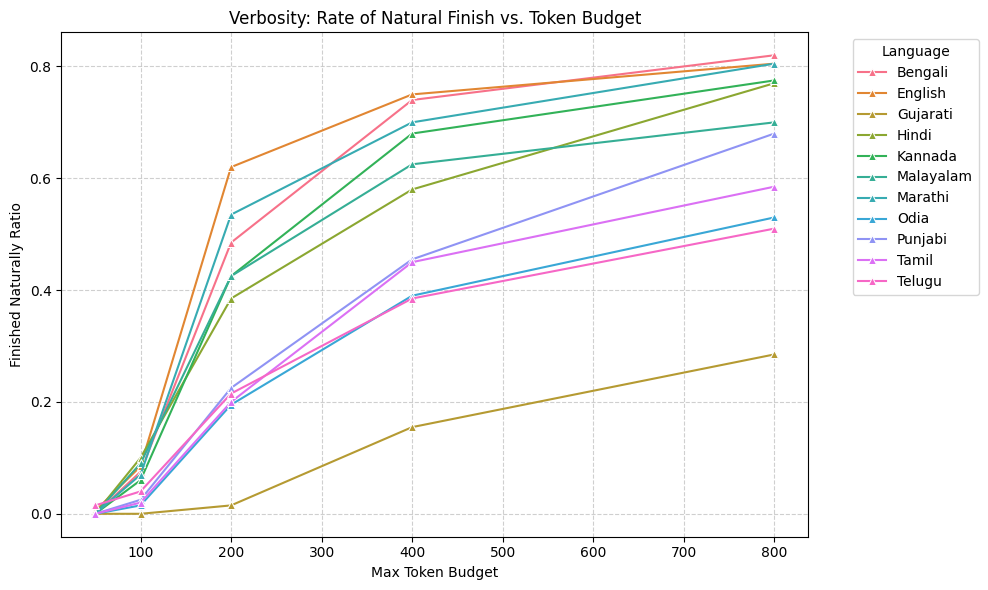
\includegraphics[
%         width=\linewidth,
%         keepaspectratio
%     ]{figures/completion_budget.jpg}
%     \caption{Natural finish rate of DeepSeek-R1-Distill-Qwen-1.5B
%     across English and ten Indic languages under five reasoning-token
%     budgets. A natural finish occurs when the model generates the
%     \texttt{</think>} marker before exhausting the reasoning-token budget.}
%     \label{fig:completion_budget}
% \end{figure}


% \subsection{Token Bloat Across Languages}

% We measure token bloat relative to English to examine differences in token usage across languages. The analysis considers generations produced under the 800-token reasoning budget that finished their thinking stage naturally. For each Indic language, we compare valid question pairs against the English condition and calculate the average token bloat multiplier. Table~\ref{tab:token_bloat} reports the number of valid comparisons and the average multiplier for each language.

% Gujarati exhibits the highest token bloat multiplier at 2.85$\times$ relative to English, based on 49 valid question comparisons. Punjabi follows at 2.46$\times$, while Telugu and Odia show multipliers of 2.17$\times$ and 2.04$\times$, respectively. Tamil has a multiplier of 2.02$\times$, and Hindi has a multiplier of 1.87$\times$. Bengali and Kannada exhibit multipliers of 1.74$\times$ and 1.72$\times$, respectively. Malayalam and Marathi have the lowest multipliers, at 1.59$\times$ and 1.54$\times$.

% These results indicate substantial differences in token usage across the evaluated languages. In the analyzed question pairs, generated thinking traces in every Indic language have a higher average token count than their English counterparts. The size of this difference varies across languages, with Gujarati showing the largest relative token cost and Marathi the smallest.

% The Gujarati result is particularly noteworthy when considered alongside the completion analysis in Section~\ref{subsec:natural_finish}. Gujarati has the highest measured token bloat multiplier and a notably low natural finish rate. One possible explanation is that greater token consumption leaves less room for completing a reasoning trace within a fixed budget. However, the current observations do not establish that token bloat causes premature cutoffs. Language-specific reasoning behavior and differences in the valid comparison sets may also contribute to the observed pattern.

% The valid comparison counts differ across languages, ranging from 49 for Gujarati to 138 for Bengali. Therefore, the reported averages are based on different numbers of question pairs. In particular, the Gujarati estimate should be interpreted with caution because it is based on fewer valid comparisons. Further analysis across matched examples and additional models will help determine whether the observed differences persist.

% Overall, the results provide evidence of a language-dependent token cost under the evaluated generation conditions. This finding motivates further investigation into how tokenization and reasoning behavior interact under constrained budgets.


% \begin{figure}[htbp]
%     \centering
%     \includegraphics[width=0.95\linewidth]
%     {figures/token_bloat.jpg}
%     \caption{Average token bloat multiplier relative to English for
%     naturally completed thinking traces under the 800-token reasoning
%     budget. The values show the average multiplier for each language,
%     with the number of valid question pairs indicated beside each bar.}
%     \label{fig:token_bloat}
% \end{figure}


% \begin{table}[t]
% \centering
% \caption{Token bloat relative to English for naturally completed
% thinking traces under the 800-token reasoning budget.}
% \label{tab:token_bloat}
% \begin{tabular}{lrr}
% \toprule
% Language & Valid Comparisons & Avg. Bloat Multiplier \\
% \midrule
% Gujarati   & 49  & 2.85$\times$ \\
% Punjabi    & 115 & 2.46$\times$ \\
% Telugu     & 85  & 2.17$\times$ \\
% Odia       & 87  & 2.04$\times$ \\
% Tamil      & 102 & 2.02$\times$ \\
% Hindi      & 125 & 1.87$\times$ \\
% Bengali    & 138 & 1.74$\times$ \\
% Kannada    & 128 & 1.72$\times$ \\
% Malayalam  & 115 & 1.59$\times$ \\
% Marathi    & 130 & 1.54$\times$ \\
% \bottomrule
% \end{tabular}
% \end{table}

% \subsection{Target-Script Usage and Mathematical Accuracy}

% We examine the relationship between target-script usage and mathematical accuracy to investigate whether generating reasoning in an Indic language's native script is associated with better performance. We use the character-level target-script ratio defined in Section~4.3 and compare it with exact-match accuracy across languages.

% Gujarati exhibits the highest target-script usage among the evaluated Indic languages. Its reasoning traces retain substantially more of the target script than those of the other Indic-language conditions. However, Gujarati also exhibits a low natural finish rate and the highest token bloat multiplier relative to English in our 800-token analysis. These findings show that greater target-script usage can coexist with a higher token cost and more frequent reasoning truncation.

% Hindi provides a useful contrast. It achieves the highest mathematical accuracy among the Indic languages, although Gujarati shows stronger target-script persistence. This difference suggests that native-script usage alone does not explain the observed accuracy ranking. Other factors, including tokenization cost and language-specific model behavior, may also contribute to performance differences.

% We further examine accuracy across groups of reasoning traces with different target-script ratios. Figure~\ref{fig:script_accuracy} will present this comparison, while Figure~\ref{fig:script_ratio} will summarize target-script usage across languages. These analyses help assess whether traces with greater target-script usage tend to achieve higher accuracy within each language.

% The target-script ratio measures the proportion of counted characters belonging to the target writing system. It does not directly identify semantic language choice or count switches between languages. Therefore, we interpret this metric as a measure of script composition rather than a direct measure of language switching.

% Taken together, the results do not support treating native-script persistence as a sufficient indicator of mathematical reasoning quality. Gujarati's high target-script usage alongside its low finish rate and high token bloat highlights the need to study script composition, tokenization cost, reasoning completion, and accuracy together. These observed relationships are descriptive and do not establish that using a native script causes either higher or lower mathematical accuracy.

% \begin{figure}[htbp]
%     \centering
%     \includegraphics[width=0.95\linewidth]
%     {figures/script_ratio.jpg}
%     \caption{Percentage of each language's thinking trace written in
%     its target script across five reasoning-token budgets.}
%     \label{fig:script_ratio}
% \end{figure}


% \begin{figure}[htbp]
%     \centering
%     \includegraphics[width=\linewidth]
%     {figures/figure6_script_accuracy_heatmap.jpg}
%     \caption{Exact-match accuracy grouped by target-script ratio for
%     English fallback and native-script reasoning traces at the
%     800-token reasoning budget. Blank cells indicate groups for which
%     no value is displayed in the supplied results.}
%     \label{fig:script_accuracy}
% \end{figure}


% \subsection{Overall Discussion}

% The experiments reveal differences in mathematical reasoning accuracy, reasoning completion, token usage, and target-script persistence across English and ten Indic languages. These results provide an initial view of how reasoning-token constraints affect DeepSeek-R1-Distill-Qwen-1.5B across languages.

% \textbf{RQ1: Effect of reasoning-token budgets.}
% English achieves the highest mathematical accuracy across the evaluated conditions. Among the Indic languages, Hindi achieves the highest accuracy. Although larger reasoning budgets improve accuracy in several languages, the gains vary across languages, and some show limited improvement as the budget increases. This suggests that increasing the available reasoning tokens does not produce uniform improvements across language conditions.

% \textbf{RQ2: Relationship between token usage and reasoning completion.}
% The token bloat analysis shows that all ten Indic languages require more tokens than English for the compared, naturally completed thinking traces. Gujarati has the highest average token bloat multiplier at 2.85$\times$, while Marathi has the lowest at 1.54$\times$. Gujarati also exhibits a notably low natural finish rate. These observations are consistent with the possibility that higher token consumption leaves less room for reasoning under a fixed budget. However, the current results establish an association rather than a causal relationship.

% \textbf{RQ3: Target-script persistence and accuracy.}
% Gujarati exhibits the strongest target-script persistence among the evaluated Indic languages, but Hindi achieves higher mathematical accuracy. This indicates that greater native-script usage does not necessarily correspond to better mathematical reasoning performance. Script composition, token consumption, and reasoning completion capture different aspects of generation and should be examined together.

% Taken together, the results show that the effect of a fixed reasoning-token budget differs across language conditions. The observed differences motivate further investigation into how tokenization cost and language-specific generation behavior contribute to mathematical reasoning performance. Since the current experiments evaluate one model, additional model evaluations are required before determining whether these patterns extend to other small language models.

% \subsection{Research Progress and Planned Evaluation}
% The current stage includes the completed evaluation of DeepSeek-R1-Distill-Qwen-1.5B across English and ten Indic languages under five reasoning-token budgets. The analysis covers exact-match accuracy, natural finish rate, character-level target-script ratio, and token bloat relative to English.

% The remaining work includes evaluating additional small language models, comparing language-specific trends across models, and refining the analysis of token usage and reasoning completion. We will also validate the consistency of the evaluation pipeline, consolidate the experimental results, and prepare the final figures and tables.

% These additional experiments will help determine whether the observed language differences are specific to the current model or recur across different model sizes and architectures.

% % ---------------------------------------------------------------
% % 6. CONCLUSION
% % ---------------------------------------------------------------
% % Instructions:
% %   - 2-3 paragraphs; a refined, forward-looking version of the abstract.
% %   - Be specific: mention actual numbers, dataset names, method names.
% %   - Do NOT simply copy-paste the abstract.
% % ---------------------------------------------------------------

% \section{Conclusion}

% This study investigates whether fixed reasoning-token budgets affect mathematical reasoning differently across English and ten Indic languages. We evaluate DeepSeek-R1-Distill-Qwen-1.5B on the Sarvam GSM8K-Indic dataset using five reasoning-token budgets, from 50 to 800 tokens. Our analysis considers mathematical accuracy, natural finish rate, target-script usage, and token bloat relative to English.

% The results reveal substantial differences across language conditions. English achieves the highest mathematical accuracy, while Hindi performs best among the evaluated Indic languages. Increasing the reasoning-token budget improves accuracy in several languages, but the magnitude of improvement varies. A larger budget therefore does not guarantee uniform gains across languages.

% Our token bloat analysis identifies additional differences in token usage. Among the evaluated Indic languages, Gujarati has the highest average token bloat multiplier relative to English, at 2.85$\times$, while Marathi has the lowest, at 1.54$\times$, for the naturally completed thinking traces analyzed under the 800-token budget. Gujarati also exhibits a notably low natural finish rate despite having the strongest target-script persistence among the Indic languages. In contrast, Hindi achieves the highest Indic-language accuracy. These findings show that target-script usage, token consumption, reasoning completion, and mathematical accuracy do not necessarily follow the same pattern.

% Overall, the findings provide initial evidence that a shared reasoning-token budget can lead to different generation and accuracy outcomes across languages. Token bloat is a plausible contributor to these differences, but the current results do not establish a causal relationship between tokenization cost and mathematical accuracy. The findings also come from a single model and should not yet be generalized to all small language models.

% Future work will evaluate additional small language models to determine whether these patterns persist across model sizes and architectures. We will also refine cross-language comparisons and further examine the relationship between token bloat, reasoning completion, target-script usage, and answer accuracy. This broader evaluation will help establish whether token-budget policies require language-sensitive considerations when applied to multilingual reasoning systems.

% % % ---------------------------------------------------------------
% % % LIMITATIONS  (mandatory for ACL/ARR)
% % % ---------------------------------------------------------------
% % \section*{Limitations}
% % \label{sec:limitations}

% % \begin{itemize}
% %     \item \textbf{Dataset limitations:}
% %     [The datasets used may not fully represent all languages, dialects, or
% %     demographic groups.
% %     Annotation quality may vary across sources, and dataset size may be
% %     insufficient for fine-grained sub-group analysis.]

% %     \item \textbf{Methodological limitations:}
% %     [Our approach assumes [assumption], which may not hold in all real-world
% %     settings.
% %     The method requires [input type] that may not always be available in
% %     practice.]

% %     \item \textbf{Model limitations:}
% %     [We evaluated models up to [X]B parameters; behaviour at larger scales
% %     is unknown.
% %     Proprietary models are accessed via API without access to weights or
% %     logits, limiting interpretability.]

% %     \item \textbf{Computational limitations:}
% %     [Full fine-tuning experiments were constrained by GPU availability.
% %     Some configurations were tested only at smaller scale due to cost
% %     constraints.]

% %     \item \textbf{Generalizability:}
% %     [Results may not generalise to low-resource languages, highly
% %     specialised domains, or task formulations significantly different from
% %     those evaluated here.]
% % \end{itemize}

% % % ---------------------------------------------------------------
% % % ACKNOWLEDGEMENTS
% % % ---------------------------------------------------------------
% % \section*{Acknowledgements}

% % [This research was supported by [Funding Agency], Grant No.\ [XXXX].
% % We thank [Name(s)] for insightful discussions and feedback on earlier
% % drafts.
% % We are grateful to [Institution / Platform] for providing computational
% % resources.
% % We also thank the anonymous reviewers for their constructive comments.]

% % \noindent\textbf{AI Use Statement.}
% % The authors are responsible for all content, facts, and claims presented
% % in this paper.
% % Any use of AI-assisted writing tools was limited to [grammar checking /
% % brainstorming / none].
% % All scientific content, analysis, results, and conclusions are entirely
% % the authors' own.

% % % ---------------------------------------------------------------
% % % REFERENCES
% % % ---------------------------------------------------------------
% % % natbib citation commands:
% % %   \citep{key}       ->  (Author, Year)
% % %   \citet{key}       ->  Author (Year)
% % %   \citealp{key}     ->  Author, Year   (inside parentheses)
% % %   \citeyearpar{key} ->  (Year)
% % %   \citeposs{key}    ->  Author's (Year)  [ACL-specific]
% % %
% % % Ensure all datasets, models, metrics, and systems are cited here.
% % % For ACL Anthology papers, download anthology.bib from:
% % %   https://aclweb.org/anthology/anthology.bib.gz
% % % ---------------------------------------------------------------

% % % Bibliography entries for the entire Anthology, followed by custom entries
% % %\bibliography{anthology,custom}
% % % Custom bibliography entries only
% % \bibliography{custom}

% % % ---------------------------------------------------------------
% % % APPENDIX
% % % ---------------------------------------------------------------
% % % Instructions:
% % %   - Appendix does NOT count toward the ACL/ARR page limit.
% % %   - Use \appendix to switch section numbering to letters (A, B, C ...).
% % %   - Common contents: full prompts, extra results, annotation guidelines,
% % %     significance tests, extended examples.
% % % ---------------------------------------------------------------
% % \appendix

% % \section{Full Prompt Templates}
% % \label{app:prompts}

% % [If your method uses prompting, include the exact prompt templates here
% % so that reviewers can verify and reproduce your work.
% % Use \texttt{verbatim} or a code-listing environment:]

% % \begin{verbatim}
% % System: You are a helpful assistant.
% % User: Given the following [INPUT TYPE]:
% % ---
% % {input}
% % ---
% % Please [TASK DESCRIPTION].
% % Output format: [SPECIFY FORMAT].
% % \end{verbatim}

% % [Add one block per distinct prompt type used in your experiments.
% % Label each clearly with its purpose --- \eg zero-shot prompt, few-shot
% % prompt, chain-of-thought prompt, etc.]

% % \section{Additional Experimental Results}
% % \label{app:extra_results}

% % [Tables or figures that support the main results but were omitted from
% % the main paper for space.
% % Each table and figure must have a caption.]

% % \begin{table}[h]
% %   \centering
% %   \small
% %   \begin{tabular}{lcccc}
% %     \hline
% %     \textbf{System} & \textbf{[DS 1]} & \textbf{[DS 2]} &
% %     \textbf{[DS 3]} & \textbf{Avg.} \\
% %     \hline
% %     [System 1] & XX.X & XX.X & XX.X & XX.X \\
% %     [System 2] & XX.X & XX.X & XX.X & XX.X \\
% %     \hline
% %   \end{tabular}
% %   \caption{Full results across all datasets and all models.}
% %   \label{tab:app_results}
% % \end{table}

% % \section{Dataset Construction Details}
% % \label{app:dataset}

% % [For benchmark or dataset papers: full annotation guidelines, quality
% % control procedures, inter-annotator agreement (IAA) scores, and annotator
% % demographics if applicable.
% % \eg ``Three trained annotators labelled each instance independently.
% % Cohen's $\kappa = X.XX$, indicating [level of] agreement.''
% % Describe any adjudication process used to resolve disagreements.]

% % \section{Statistical Significance Tests}
% % \label{app:significance}

% % [Report the statistical test used (\eg bootstrap resampling, paired
% % $t$-test, Wilcoxon signed-rank), the significance threshold ($p < 0.05$),
% % and which comparisons are significant.
% % A full pairwise significance table is recommended here.]

% % \begin{table}[h]
% %   \centering
% %   \small
% %   \begin{tabular}{lcc}
% %     \hline
% %     \textbf{Comparison} & \textbf{[Metric 1]} & \textbf{[Metric 2]} \\
% %     \hline
% %     Ours vs.\ Baseline 1 & $<$0.01\ $\checkmark$ & $<$0.05\ $\checkmark$ \\
% %     Ours vs.\ Baseline 2 & $<$0.05\ $\checkmark$ & 0.12 \\
% %     Ours vs.\ Baseline 3 & $<$0.01\ $\checkmark$ & $<$0.01\ $\checkmark$ \\
% %     \hline
% %   \end{tabular}
% %   \caption{Pairwise statistical significance ($p$-values).
% %     $\checkmark$ = $p < 0.05$.}
% %   \label{tab:significance}
% % \end{table}

% % \section{Extended Qualitative Examples}
% % \label{app:examples}

% % [Additional input/output examples illustrating system behaviour across
% % diverse conditions, including both success cases and failure modes.
% % The four-column table format below --- Input, Gold Label, Best Baseline
% % Output, Your System Output --- works well for most NLP tasks.]

% % \begin{table*}[h]
% %   \centering
% %   \small
% %   \begin{tabularx}{\textwidth}{lXXXc}
% %     \hline
% %     \textbf{ID} & \textbf{Input} & \textbf{Gold} &
% %     \textbf{Best Baseline} & \textbf{Ours} \\
% %     \hline
% %     1 & [Input 1] & [Gold] & [Output -- incorrect] &
% %       [Output -- correct] \\
% %     2 & [Input 2] & [Gold] & [Output -- correct] &
% %       [Output -- correct] \\
% %     3 & [Input 3 --- failure case] & [Gold] & [Output -- incorrect] &
% %       [Output -- incorrect] \\
% %     \hline
% %   \end{tabularx}
% %   \caption{Extended qualitative examples showing success and failure cases.}
% %   \label{tab:examples}
% % \end{table*}

% \end{document}

% % % ===============================================================
% % %  END OF DOCUMENT
% % %  ACL / ARR Research Paper Skeleton v1.0
% % %  Replace all [bracketed placeholders] with your specific content.
% % %  Compile order: pdflatex -> bibtex -> pdflatex -> pdflatex
% % %  On Overleaf: upload acl.sty, acl_natbib.bst, and your custom.bib
% % % ===============================================================



% % % \documentclass[11pt]{article}

% % % % Change "review" to "final" to generate the final (sometimes called camera-ready) version.
% % % % Change to "preprint" to generate a non-anonymous version with page numbers.
% % % \usepackage[review]{acl}

% % % % Standard package includes
% % % \usepackage{times}
% % % \usepackage{latexsym}

% % % % For proper rendering and hyphenation of words containing Latin characters (including in bib files)
% % % \usepackage[T1]{fontenc}
% % % % For Vietnamese characters
% % % % \usepackage[T5]{fontenc}
% % % % See https://www.latex-project.org/help/documentation/encguide.pdf for other character sets

% % % % This assumes your files are encoded as UTF8
% % % \usepackage[utf8]{inputenc}

% % % % This is not strictly necessary, and may be commented out,
% % % % but it will improve the layout of the manuscript,
% % % % and will typically save some space.
% % % \usepackage{microtype}

% % % % This is also not strictly necessary, and may be commented out.
% % % % However, it will improve the aesthetics of text in
% % % % the typewriter font.
% % % \usepackage{inconsolata}

% % % %Including images in your LaTeX document requires adding
% % % %additional package(s)
% % % \usepackage{graphicx}

% % % % If the title and author information does not fit in the area allocated, uncomment the following
% % % %
% % % %\setlength\titlebox{<dim>}
% % % %
% % % % and set <dim> to something 5cm or larger.

% % % \title{Instructions for *ACL Proceedings}

% % % % Author information can be set in various styles:
% % % % For several authors from the same institution:
% % % % \author{Author 1 \and ... \and Author n \\
% % % %         Address line \\ ... \\ Address line}
% % % % if the names do not fit well on one line use
% % % %         Author 1 \\ {\bf Author 2} \\ ... \\ {\bf Author n} \\
% % % % For authors from different institutions:
% % % % \author{Author 1 \\ Address line \\  ... \\ Address line
% % % %         \And  ... \And
% % % %         Author n \\ Address line \\ ... \\ Address line}
% % % % To start a separate ``row'' of authors use \AND, as in
% % % % \author{Author 1 \\ Address line \\  ... \\ Address line
% % % %         \AND
% % % %         Author 2 \\ Address line \\ ... \\ Address line \And
% % % %         Author 3 \\ Address line \\ ... \\ Address line}

% % % \author{First Author \\
% % %   Affiliation / Address line 1 \\
% % %   Affiliation / Address line 2 \\
% % %   Affiliation / Address line 3 \\
% % %   \texttt{email@domain} \\\And
% % %   Second Author \\
% % %   Affiliation / Address line 1 \\
% % %   Affiliation / Address line 2 \\
% % %   Affiliation / Address line 3 \\
% % %   \texttt{email@domain} \\}

% % % %\author{
% % % %  \textbf{First Author\textsuperscript{1}},
% % % %  \textbf{Second Author\textsuperscript{1,2}},
% % % %  \textbf{Third T. Author\textsuperscript{1}},
% % % %  \textbf{Fourth Author\textsuperscript{1}},
% % % %\\
% % % %  \textbf{Fifth Author\textsuperscript{1,2}},
% % % %  \textbf{Sixth Author\textsuperscript{1}},
% % % %  \textbf{Seventh Author\textsuperscript{1}},
% % % %  \textbf{Eighth Author \textsuperscript{1,2,3,4}},
% % % %\\
% % % %  \textbf{Ninth Author\textsuperscript{1}},
% % % %  \textbf{Tenth Author\textsuperscript{1}},
% % % %  \textbf{Eleventh E. Author\textsuperscript{1,2,3,4,5}},
% % % %  \textbf{Twelfth Author\textsuperscript{1}},
% % % %\\
% % % %  \textbf{Thirteenth Author\textsuperscript{3}},
% % % %  \textbf{Fourteenth F. Author\textsuperscript{2,4}},
% % % %  \textbf{Fifteenth Author\textsuperscript{1}},
% % % %  \textbf{Sixteenth Author\textsuperscript{1}},
% % % %\\
% % % %  \textbf{Seventeenth S. Author\textsuperscript{4,5}},
% % % %  \textbf{Eighteenth Author\textsuperscript{3,4}},
% % % %  \textbf{Nineteenth N. Author\textsuperscript{2,5}},
% % % %  \textbf{Twentieth Author\textsuperscript{1}}
% % % %\\
% % % %\\
% % % %  \textsuperscript{1}Affiliation 1,
% % % %  \textsuperscript{2}Affiliation 2,
% % % %  \textsuperscript{3}Affiliation 3,
% % % %  \textsuperscript{4}Affiliation 4,
% % % %  \textsuperscript{5}Affiliation 5
% % % %\\
% % % %  \small{
% % % %    \textbf{Correspondence:} \href{mailto:email@domain}{email@domain}
% % % %  }
% % % %}

% % % \begin{document}
% % % \maketitle
% % % \begin{abstract}
% % % This document is a supplement to the general instructions for *ACL authors. It contains instructions for using the \LaTeX{} style files for ACL conferences.
% % % The document itself conforms to its own specifications, and is therefore an example of what your manuscript should look like.
% % % These instructions should be used both for papers submitted for review and for final versions of accepted papers.
% % % \end{abstract}

% % % \section{Introduction}

% % % These instructions are for authors submitting papers to *ACL conferences using \LaTeX. They are not self-contained. All authors must follow the general instructions for *ACL proceedings,\footnote{\url{http://acl-org.github.io/ACLPUB/formatting.html}} and this document contains additional instructions for the \LaTeX{} style files.

% % % The templates include the \LaTeX{} source of this document (\texttt{acl\_latex.tex}),
% % % the \LaTeX{} style file used to format it (\texttt{acl.sty}),
% % % an ACL bibliography style (\texttt{acl\_natbib.bst}),
% % % an example bibliography (\texttt{custom.bib}),
% % % and the bibliography for the ACL Anthology (\texttt{anthology.bib}).

% % % \section{Engines}

% % % To produce a PDF file, pdf\LaTeX{} is strongly recommended (over original \LaTeX{} plus dvips+ps2pdf or dvipdf).
% % % The style file \texttt{acl.sty} can also be used with
% % % lua\LaTeX{} and
% % % Xe\LaTeX{}, which are especially suitable for text in non-Latin scripts.
% % % The file \texttt{acl\_lualatex.tex} in this repository provides
% % % an example of how to use \texttt{acl.sty} with either
% % % lua\LaTeX{} or
% % % Xe\LaTeX{}.

% % % \section{Preamble}

% % % The first line of the file must be
% % % \begin{quote}
% % % \begin{verbatim}
% % % \documentclass[11pt]{article}
% % % \end{verbatim}
% % % \end{quote}

% % % To load the style file in the review version:
% % % \begin{quote}
% % % \begin{verbatim}
% % % \usepackage[review]{acl}
% % % \end{verbatim}
% % % \end{quote}
% % % For the final version, omit the \verb|review| option:
% % % \begin{quote}
% % % \begin{verbatim}
% % % \usepackage{acl}
% % % \end{verbatim}
% % % \end{quote}

% % % To use Times Roman, put the following in the preamble:
% % % \begin{quote}
% % % \begin{verbatim}
% % % \usepackage{times}
% % % \end{verbatim}
% % % \end{quote}
% % % (Alternatives like txfonts or newtx are also acceptable.)

% % % Please see the \LaTeX{} source of this document for comments on other packages that may be useful.

% % % Set the title and author using \verb|\title| and \verb|\author|. Within the author list, format multiple authors using \verb|\and| and \verb|\And| and \verb|\AND|; please see the \LaTeX{} source for examples.

% % % By default, the box containing the title and author names is set to the minimum of 5 cm. If you need more space, include the following in the preamble:
% % % \begin{quote}
% % % \begin{verbatim}
% % % \setlength\titlebox{<dim>}
% % % \end{verbatim}
% % % \end{quote}
% % % where \verb|<dim>| is replaced with a length. Do not set this length smaller than 5 cm.

% % % \section{Document Body}

% % % \subsection{Footnotes}

% % % Footnotes are inserted with the \verb|\footnote| command.\footnote{This is a footnote.}

% % % \subsection{Tables and figures}

% % % See Table~\ref{tab:accents} for an example of a table and its caption.
% % % \textbf{Do not override the default caption sizes.}

% % % \begin{table}
% % %   \centering
% % %   \begin{tabular}{lc}
% % %     \hline
% % %     \textbf{Command} & \textbf{Output} \\
% % %     \hline
% % %     \verb|{\"a}|     & {\"a}           \\
% % %     \verb|{\^e}|     & {\^e}           \\
% % %     \verb|{\`i}|     & {\`i}           \\
% % %     \verb|{\.I}|     & {\.I}           \\
% % %     \verb|{\o}|      & {\o}            \\
% % %     \verb|{\'u}|     & {\'u}           \\
% % %     \verb|{\aa}|     & {\aa}           \\\hline
% % %   \end{tabular}
% % %   \begin{tabular}{lc}
% % %     \hline
% % %     \textbf{Command} & \textbf{Output} \\
% % %     \hline
% % %     \verb|{\c c}|    & {\c c}          \\
% % %     \verb|{\u g}|    & {\u g}          \\
% % %     \verb|{\l}|      & {\l}            \\
% % %     \verb|{\~n}|     & {\~n}           \\
% % %     \verb|{\H o}|    & {\H o}          \\
% % %     \verb|{\v r}|    & {\v r}          \\
% % %     \verb|{\ss}|     & {\ss}           \\
% % %     \hline
% % %   \end{tabular}
% % %   \caption{Example commands for accented characters, to be used in, \emph{e.g.}, Bib\TeX{} entries.}
% % %   \label{tab:accents}
% % % \end{table}

% % % As much as possible, fonts in figures should conform
% % % to the document fonts. See Figure~\ref{fig:experiments} for an example of a figure and its caption.

% % % Using the \verb|graphicx| package graphics files can be included within figure
% % % environment at an appropriate point within the text.
% % % The \verb|graphicx| package supports various optional arguments to control the
% % % appearance of the figure.
% % % You must include it explicitly in the \LaTeX{} preamble (after the
% % % \verb|\documentclass| declaration and before \verb|\begin{document}|) using
% % % \verb|\usepackage{graphicx}|.

% % % \begin{figure}[t]
% % %   \includegraphics[width=\columnwidth]{example-image-golden}
% % %   \caption{A figure with a caption that runs for more than one line.
% % %     Example image is usually available through the \texttt{mwe} package
% % %     without even mentioning it in the preamble.}
% % %   \label{fig:experiments}
% % % \end{figure}

% % % \begin{figure*}[t]
% % %   \includegraphics[width=0.48\linewidth]{example-image-a} \hfill
% % %   \includegraphics[width=0.48\linewidth]{example-image-b}
% % %   \caption {A minimal working example to demonstrate how to place
% % %     two images side-by-side.}
% % % \end{figure*}

% % % \subsection{Hyperlinks}

% % % Users of older versions of \LaTeX{} may encounter the following error during compilation:
% % % \begin{quote}
% % % \verb|\pdfendlink| ended up in different nesting level than \verb|\pdfstartlink|.
% % % \end{quote}
% % % This happens when pdf\LaTeX{} is used and a citation splits across a page boundary. The best way to fix this is to upgrade \LaTeX{} to 2018-12-01 or later.

% % % \subsection{Citations}

% % % \begin{table*}
% % %   \centering
% % %   \begin{tabular}{lll}
% % %     \hline
% % %     \textbf{Output}           & \textbf{natbib command} & \textbf{ACL only command} \\
% % %     \hline
% % %     \citep{Gusfield:97}       & \verb|\citep|           &                           \\
% % %     \citealp{Gusfield:97}     & \verb|\citealp|         &                           \\
% % %     \citet{Gusfield:97}       & \verb|\citet|           &                           \\
% % %     \citeyearpar{Gusfield:97} & \verb|\citeyearpar|     &                           \\
% % %     \citeposs{Gusfield:97}    &                         & \verb|\citeposs|          \\
% % %     \hline
% % %   \end{tabular}
% % %   \caption{\label{citation-guide}
% % %     Citation commands supported by the style file.
% % %     The style is based on the natbib package and supports all natbib citation commands.
% % %     It also supports commands defined in previous ACL style files for compatibility.
% % %   }
% % % \end{table*}

% % % Table~\ref{citation-guide} shows the syntax supported by the style files.
% % % We encourage you to use the natbib styles.
% % % You can use the command \verb|\citet| (cite in text) to get ``author (year)'' citations, like this citation to a paper by \citet{Gusfield:97}.
% % % You can use the command \verb|\citep| (cite in parentheses) to get ``(author, year)'' citations \citep{Gusfield:97}.
% % % You can use the command \verb|\citealp| (alternative cite without parentheses) to get ``author, year'' citations, which is useful for using citations within parentheses (e.g. \citealp{Gusfield:97}).

% % % A possessive citation can be made with the command \verb|\citeposs|.
% % % This is not a standard natbib command, so it is generally not compatible
% % % with other style files.

% % \subsection{References}

% % % \nocite{Ando2005,andrew2007scalable,rasooli-tetrault-2015}

% % % The \LaTeX{} and Bib\TeX{} style files provided roughly follow the American Psychological Association format.
% % % If your own bib file is named \texttt{custom.bib}, then placing the following before any appendices in your \LaTeX{} file will generate the references section for you:
% % % \begin{quote}
% % % \begin{verbatim}
% % % \bibliography{custom}
% % % \end{verbatim}
% % % \end{quote}

% % % You can obtain the complete ACL Anthology as a Bib\TeX{} file from \url{https://aclweb.org/anthology/anthology.bib.gz}.
% % % To include both the Anthology and your own .bib file, use the following instead of the above.
% % % \begin{quote}
% % % \begin{verbatim}
% % % \bibliography{anthology,custom}
% % % \end{verbatim}
% % % \end{quote}

% % % Please see Section~\ref{sec:bibtex} for information on preparing Bib\TeX{} files.

% % % \subsection{Equations}

% % % An example equation is shown below:
% % % \begin{equation}
% % %   \label{eq:example}
% % %   A = \pi r^2
% % % \end{equation}

% % % Labels for equation numbers, sections, subsections, figures and tables
% % % are all defined with the \verb|\label{label}| command and cross references
% % % to them are made with the \verb|\ref{label}| command.

% % % This an example cross-reference to Equation~\ref{eq:example}.

% % % \subsection{Appendices}

% % % Use \verb|\appendix| before any appendix section to switch the section numbering over to letters. See Appendix~\ref{sec:appendix} for an example.

% % % \section{Bib\TeX{} Files}
% % % \label{sec:bibtex}

% % % Unicode cannot be used in Bib\TeX{} entries, and some ways of typing special characters can disrupt Bib\TeX's alphabetization. The recommended way of typing special characters is shown in Table~\ref{tab:accents}.

% % % Please ensure that Bib\TeX{} records contain DOIs or URLs when possible, and for all the ACL materials that you reference.
% % % Use the \verb|doi| field for DOIs and the \verb|url| field for URLs.
% % % If a Bib\TeX{} entry has a URL or DOI field, the paper title in the references section will appear as a hyperlink to the paper, using the hyperref \LaTeX{} package.

% % % \section*{Limitations}

% % % This document does not cover the content requirements for ACL or any
% % % other specific venue.  Check the author instructions for
% % % information on
% % % maximum page lengths, the required ``Limitations'' section,
% % % and so on.

% % % \section*{Acknowledgments}

% % % This document has been adapted
% % % by Steven Bethard, Ryan Cotterell and Rui Yan
% % % from the instructions for earlier ACL and NAACL proceedings, including those for
% % % ACL 2019 by Douwe Kiela and Ivan Vuli\'{c},
% % % NAACL 2019 by Stephanie Lukin and Alla Roskovskaya,
% % % ACL 2018 by Shay Cohen, Kevin Gimpel, and Wei Lu,
% % % NAACL 2018 by Margaret Mitchell and Stephanie Lukin,
% % % Bib\TeX{} suggestions for (NA)ACL 2017/2018 from Jason Eisner,
% % % ACL 2017 by Dan Gildea and Min-Yen Kan,
% % % NAACL 2017 by Margaret Mitchell,
% % % ACL 2012 by Maggie Li and Michael White,
% % % ACL 2010 by Jing-Shin Chang and Philipp Koehn,
% % % ACL 2008 by Johanna D. Moore, Simone Teufel, James Allan, and Sadaoki Furui,
% % % ACL 2005 by Hwee Tou Ng and Kemal Oflazer,
% % % ACL 2002 by Eugene Charniak and Dekang Lin,
% % % and earlier ACL and EACL formats written by several people, including
% % % John Chen, Henry S. Thompson and Donald Walker.
% % % Additional elements were taken from the formatting instructions of the \emph{International Joint Conference on Artificial Intelligence} and the \emph{Conference on Computer Vision and Pattern Recognition}.

% % % % Bibliography entries for the entire Anthology, followed by custom entries
% % % \bibliography{anthology,custom}
% % % % Custom bibliography entries only
% % % \bibliography{custom}

% % % \appendix

% % % \section{Example Appendix}
% % % \label{sec:appendix}

% % % This is an appendix.

% % % \end{document}

